\documentclass[11pt]{amsart}
\usepackage[T1]{fontenc}
\usepackage{lmodern}
\usepackage[margin=1.1in]{geometry}
\usepackage{amsmath,amssymb,amsthm,mathtools}
\usepackage{enumitem}
\usepackage{booktabs,array}
\usepackage{tikz}
\usetikzlibrary{arrows.meta,positioning,decorations.pathreplacing,calc}
\usepackage{microtype}
\usepackage{xurl}
\usepackage[colorlinks=true,linkcolor=blue!50!black,citecolor=green!35!black,urlcolor=blue!60!black]{hyperref}
\hypersetup{pdftitle={The Double Midset Conjecture for Metric Continua},pdfauthor={Lucas Alves de Almeida}}
\setlength{\emergencystretch}{2em}

% ---------- theorem environments ----------
\newtheorem{maintheorem}{Theorem}
\renewcommand{\themaintheorem}{\Alph{maintheorem}}
\newtheorem{theorem}{Theorem}[section]
\newtheorem{lemma}[theorem]{Lemma}
\newtheorem{proposition}[theorem]{Proposition}
\newtheorem{corollary}[theorem]{Corollary}
\newtheorem{conjecture}[theorem]{Conjecture}
\newtheorem{question}[theorem]{Question}
\theoremstyle{definition}
\newtheorem{definition}[theorem]{Definition}
\newtheorem{convention}[theorem]{Convention}
\newtheorem{fact}[theorem]{Fact}
\theoremstyle{remark}
\newtheorem{remark}[theorem]{Remark}
\newtheorem*{role}{Role in the proof}

% ---------- notation ----------
\newcommand{\M}{M}
\newcommand{\Odd}{O}
\newcommand{\Ver}{V}
\newcommand{\N}{N}
\newcommand{\sgn}{\operatorname{sgn}}
\newcommand{\diam}{\operatorname{diam}}
\newcommand{\cl}{\operatorname{cl}}
\newcommand{\inter}{\operatorname{int}}

\title{The Double Midset Conjecture for Metric Continua}
\author{Lucas Alves de Almeida}
\email{lucasderiva8x@gmail.com}
\subjclass[2020]{Primary 54F15, 54E35; Secondary 54F50, 51K05}
\keywords{midset, equidistant set, bisector, double midset property, metric continuum, dendrite, finite tree, simple closed curve}
\date{22 November 2026}

\begin{document}

\begin{abstract}
Let $(X,d)$ be a nondegenerate compact connected metric space such that, for any two distinct points $a,b\in X$, exactly two points of $X$ are equidistant from $a$ and $b$. We prove that $X$ is homeomorphic to a circle. This settles the double midset conjecture of Loveland and Wayment from 1974. It was previously known for plane continua with the Euclidean metric and under additional convexity or continuity hypotheses. No assumption on the metric is made beyond compatibility with the topology. We first show that a counterexample would be a finite tree. On a finite tree, a parity count of the sign changes of $d(\cdot,a)-d(\cdot,b)$, combined with a Baire category argument, forces whole intervals onto metric spheres. This rigidity is incompatible with a branch point and with an arc. The results of the paper are formalized in Lean~4.
\end{abstract}

\maketitle
\setcounter{tocdepth}{1}
\tableofcontents

% =====================================================================
\section{Introduction}\label{sec:intro}

\subsection{The conjecture}
Let $(X,d)$ be a metric space. For distinct points $a,b\in X$ (the \emph{sites}), the \emph{midset}, also called the equidistant set or bisector, of $a$ and $b$ is
\[
  \M(a,b)=\{x\in X:\ d(x,a)=d(x,b)\}.
\]
The space has the \emph{double midset property} (DMP) if $|\M(a,b)|=2$ for all distinct $a,b\in X$. The basic example is a Euclidean circle. There $\M(a,b)$ consists of the two points where the perpendicular bisector of the chord $ab$ meets the circle. The property is purely metric and is not preserved by a change to an equivalent metric. A space homeomorphic to a circle may carry metrics with and without the DMP. Connectedness cannot be dropped: four points at mutual distance one form a space with the DMP \cite[p.~347]{L76b}.

\begin{conjecture}[Loveland--Wayment \cite{LW74}; see {\cite[p.~342]{L76b}}]\label{conj:LW}
Every nondegenerate compact connected metric space with the double midset property is homeomorphic to the circle $S^1$.
\end{conjecture}

Midsets were used to characterize classical spaces long before this conjecture was formulated. Berard characterized intervals among metric spaces by means of their midsets \cite{Ber71}. Loveland and Valentine proved that a complete convex metric space with the DMP is isometric to a circle with its geodesic metric \cite[Theorem~2]{LV73}, and they later gave a short proof \cite{LV75}. Berard and Nitka obtained the same conclusion for segment-convex spaces \cite{BN74}. Convexity supplies geodesic arcs between pairs of points. An arbitrary compatible metric on a continuum has no such arcs. This is the setting of Conjecture~\ref{conj:LW}.

Loveland and Wayment \cite{LW74} proved that a continuum with the DMP that contains a nondegenerate subcontinuum without cut points is a simple closed curve; see \cite[Theorem~6]{H01}. Loveland proved the conjecture when the midset map $(a,b)\mapsto\M(a,b)$ is continuous \cite[Theorem~3]{L76}; see also \cite[Theorem~3.4]{L76b}. Loveland and Wayment showed that a continuum with finite midsets is locally connected \cite[Lemma~2]{LW74}, and Loveland extended this to Apollonius sets \cite[Lemma~2.2]{L76b}. In 1991 he proved the conjecture for subcontinua of the Euclidean plane with the inherited metric \cite{L91}. L.~D.\ and S.~M.\ Loveland showed that no plane continuum containing a simple triod has finite midsets of constant cardinality \cite[Theorem~3.1]{LL92}. Hattori's survey records the general conjecture as open \cite[p.~158]{H01}. Charatonik and Charatonik constructed a bounded planar generalized Mazurkiewicz set that is neither compact nor connected; every such set has two-point midsets \cite{CC00}. Such sets are therefore not counterexamples to Conjecture~\ref{conj:LW}; since they fail both hypotheses at once, they do not by themselves show that either hypothesis is needed separately.

\subsection{Main results}
We prove the conjecture in full generality.

\begin{maintheorem}\label{thm:A}
Let $(X,d)$ be a nondegenerate compact connected metric space. If $|\M(a,b)|=2$ for all distinct $a,b\in X$, then $X$ is homeomorphic to $S^1$. Consequently, a nondegenerate metrizable continuum admits a compatible metric with the double midset property if and only if it is a simple closed curve.
\end{maintheorem}

The proof passes through two results that may be of independent interest. The first excludes all finite trees.

\begin{maintheorem}\label{thm:B}
No finite tree admits a compatible metric with the double midset property. In particular, neither an arc nor a simple triod does.
\end{maintheorem}

The second uses only the upper bound $|\M(a,b)|\le2$.

\begin{maintheorem}\label{thm:C}
Let $X$ be a dendrite with a compatible metric such that $|\M(a,b)|\le2$ for all distinct $a,b\in X$. Then every point of $X$ has order at most four. If $X$ has a branch point of order $m$, then the set $B$ of branch points satisfies $(m-2)(|B|-1)\le m$. In particular $|B|\le4$, and $X$ is a finite tree.
\end{maintheorem}

For completeness we also include a short proof of the local connectedness result of Loveland and Wayment (Proposition~\ref{prop:lc}).

\subsection{Strategy of the proof}
Figure~\ref{fig:roadmap} shows the logical structure. For sites $a\neq b$ consider the function
\[
  f_{a,b}(y)=d(y,a)-d(y,b),\qquad y\in X .
\]
It is negative at $a$, positive at $b$, and its zero set is $\M(a,b)$.

\emph{Reduction to finite trees} (Sections~\ref{sec:dendrite}--\ref{sec:branch}). Finite midsets force local connectedness. A circle inside $X$ must be all of $X$. Hence a counterexample is a dendrite. At a branch point $c$ we perturb a site slightly. This shows that $d(c,\cdot)$ cannot decrease along arcs leaving $c$, and then that only finitely many branch points exist. This part uses only $|\M|\le2$.

\emph{Parity on a finite tree} (Section~\ref{sec:signs}). Call a zero of $f_{a,b}$ in an edge a \emph{crossing} if the sign of $f_{a,b}$ changes there and a \emph{touch} otherwise. Counting sign changes edge by edge shows that the number of crossings has the same parity as the number of odd-degree vertices where $f_{a,b}<0$. With only two zeros, a pair of odd parity has exactly one crossing and one touch.

\emph{Touches force spheres} (Section~\ref{sec:spheres}). A touch is fragile. Moving a site slightly in the wrong direction would split it into two zeros, and together with the crossing there would be three. So each site is a local extremum of the distance from the touch. A Baire category argument shows that the touch is the same point $c$ for a whole open family of pairs. All these sites then lie on one metric sphere $\{d(c,\cdot)=r\}$. Spheres containing arcs are rigid: every other observer sees such an arc strictly monotonically, and the center is unique.

\emph{Locating the center} (Sections~\ref{sec:centers}--\ref{sec:tips}). The center of a spherical arc cannot be a tip (an end) of the tree, and it cannot lie in the edge carrying the arc. With this, the distance from each end is strictly monotone on every edge. Ties through a branch point $v$ are then seen by $v$ itself.

\emph{Counting} (Sections~\ref{sec:count}--\ref{sec:arc}). Two tips cannot rise or fall together along the same pair of edges at a branch point, so a branched tree has at most three tips and is a simple triod. On the triod, the directions of change of the three end distances produce a cyclic chain of strict inequalities $r_1>r_2>r_3>r_1$ between the leg lengths $r_i=d(v,e_i)$. Finally, on an arc, alternately matching distances to the two tips produces a pair of sites with three equidistant points.

\begin{figure}[ht]
\centering
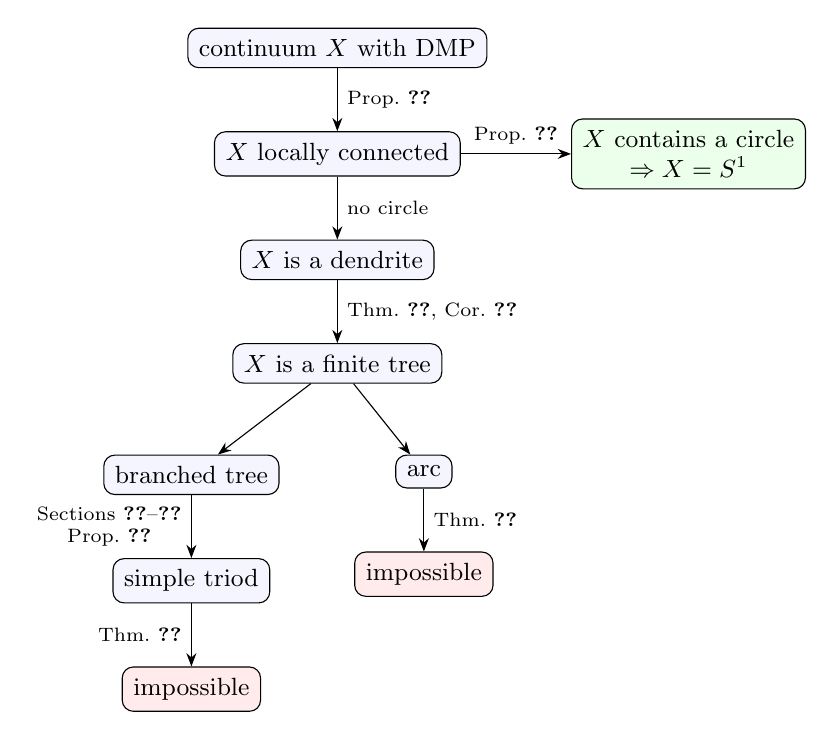
\begin{tikzpicture}[
  box/.style={draw,rounded corners,align=center,font=\small,inner sep=4pt,fill=blue!4},
  bad/.style={draw,rounded corners,align=center,font=\small,inner sep=4pt,fill=red!8},
  good/.style={draw,rounded corners,align=center,font=\small,inner sep=4pt,fill=green!8},
  lab/.style={font=\scriptsize,align=center},
  >=Stealth]
\node[box] (X) {continuum $X$ with DMP};
\node[box,below=8mm of X] (lc) {$X$ locally connected};
\node[good,right=14mm of lc] (circ) {$X$ contains a circle\\ $\Rightarrow X=S^1$};
\node[box,below=8mm of lc] (den) {$X$ is a dendrite};
\node[box,below=8mm of den] (tree) {$X$ is a finite tree};
\node[box,below left=9mm and -6mm of tree] (br) {branched tree};
\node[box,below right=9mm and -6mm of tree] (arc) {arc};
\node[box,below=8mm of br] (triod) {simple triod};
\node[bad,below=8mm of triod] (no1) {impossible};
\node[bad,below=8mm of arc] (no2) {impossible};
\draw[->] (X) -- node[lab,right]{Prop.~\ref{prop:lc}} (lc);
\draw[->] (lc) -- node[lab,above]{Prop.~\ref{prop:circle}} (circ);
\draw[->] (lc) -- node[lab,right]{no circle} (den);
\draw[->] (den) -- node[lab,right]{Thm.~\ref{thm:branchcount}, Cor.~\ref{cor:finitetree}} (tree);
\draw[->] (tree) -- (br);
\draw[->] (tree) -- (arc);
\draw[->] (br) -- node[lab,left]{Sections~\ref{sec:signs}--\ref{sec:count}\\ Prop.~\ref{prop:triod}} (triod);
\draw[->] (triod) -- node[lab,left]{Thm.~\ref{thm:triod}} (no1);
\draw[->] (arc) -- node[lab,right]{Thm.~\ref{thm:arc}} (no2);
\end{tikzpicture}
\caption{Structure of the proof of Theorem~\ref{thm:A}. Sections~\ref{sec:signs}--\ref{sec:centers} supply the common tools for both branches at the bottom.}\label{fig:roadmap}
\end{figure}

\subsection{Organization}
Section~\ref{sec:prelim} fixes notation and collects the facts from continuum theory that we use, with exact references. Section~\ref{sec:dendrite} reduces the problem to dendrites. Section~\ref{sec:branch} proves Theorem~\ref{thm:C}. Sections~\ref{sec:signs}--\ref{sec:count} develop the analysis on a finite tree: parity, spherical arcs, odd boxes, the location of centers, distances to tips, and the count of tips. Section~\ref{sec:triod} treats the simple triod and Section~\ref{sec:arc} the arc. Section~\ref{sec:proofs} assembles the proofs of Theorems~\ref{thm:A}--\ref{thm:C}. Section~\ref{sec:remarks} records which hypotheses are used where, poses some questions, and discusses the higher-dimensional $(n-1)$-sphere midset conjecture. The Lean~4 formalization of the paper is described at the end, before the references.

% =====================================================================
\subsection{Logical dependencies}
The table lists, for each result from Section~\ref{sec:dendrite} on, the earlier results it uses and the hypotheses it needs. Here ``$\le2$'' means $|\M(a,b)|\le2$ for all pairs, and ``DMP'' means $|\M(a,b)|=2$. All results from Section~\ref{sec:signs} on concern a finite tree $T$.
\begin{center}
\small
\begin{tabular}{@{}p{0.28\textwidth}p{0.42\textwidth}p{0.22\textwidth}@{}}
\toprule
Result & Uses & Hypotheses\\
\midrule
Prop.~\ref{prop:lc} & \cite[Thm.~25.3]{Mun00}, \cite[Thm.~5.6]{Nad92} & finite midsets\\
Prop.~\ref{prop:circle} & --- & $\le2$\\
Lem.~\ref{lem:radial}, \ref{lem:order} & Lem.~\ref{lem:count}, \ref{lem:extrema}, \ref{lem:arms} & $\le2$, dendrite\\
Thm.~\ref{thm:branchcount}, Cor.~\ref{cor:finitetree} & Lem.~\ref{lem:treestructure}, \ref{lem:radial}, \ref{lem:order} & $\le2$, dendrite\\
Lem.~\ref{lem:parity} & Lem.~\ref{lem:treestructure} & finitely many zeros\\
Cor.~\ref{cor:types}, Lem.~\ref{lem:stability} & Lem.~\ref{lem:count}, \ref{lem:parity} & DMP\\
Lem.~\ref{lem:sphericalarc} & Lem.~\ref{lem:separate}, \ref{lem:treestructure} & $\le2$\\
Lem.~\ref{lem:offsphere} & Cor.~\ref{cor:types}, Lem.~\ref{lem:stability}, \ref{lem:sphericalarc} & DMP\\
Prop.~\ref{prop:oddbox}, Lem.~\ref{lem:selection}, Cor.~\ref{cor:oddpair} & Lem.~\ref{lem:extrema}, \ref{lem:grid}, Cor.~\ref{cor:types}, Lem.~\ref{lem:stability}, \ref{lem:sphericalarc}, \ref{lem:offsphere} & DMP\\
Lem.~\ref{lem:tips} & Lem.~\ref{lem:parity}, \ref{lem:sphericalarc}, \ref{lem:offsphere} & DMP\\
Lem.~\ref{lem:crossing} & Cor.~\ref{cor:types}, Lem.~\ref{lem:sphericalarc}, \ref{lem:offsphere} & DMP\\
Lem.~\ref{lem:matching} & Lem.~\ref{lem:count}, \ref{lem:offsphere}, \ref{lem:crossing} & DMP\\
Lem.~\ref{lem:ownedge} & Lem.~\ref{lem:radial}, \ref{lem:crossing}, \ref{lem:matching} & DMP, branched\\
Lem.~\ref{lem:boundary} & Lem.~\ref{lem:sphericalarc}, Cor.~\ref{cor:oddpair}, Lem.~\ref{lem:ownedge} & DMP, branched\\
Prop.~\ref{prop:tipdistance} & Lem.~\ref{lem:extrema}, \ref{lem:tips}, \ref{lem:boundary} & DMP, branched\\
Lem.~\ref{lem:pairs}, Prop.~\ref{prop:triod} & Lem.~\ref{lem:radial}, \ref{lem:order}, Prop.~\ref{prop:tipdistance} & DMP, branched\\
Thm.~\ref{thm:triod} & Lem.~\ref{lem:radial}, \ref{lem:sphericalarc}, Cor.~\ref{cor:oddpair}, Lem.~\ref{lem:crossing}, Prop.~\ref{prop:tipdistance}, Lem.~\ref{lem:pairs} & DMP, simple triod\\
Thm.~\ref{thm:arc} & Lem.~\ref{lem:offsphere}, Cor.~\ref{cor:oddpair}, Lem.~\ref{lem:crossing}, \ref{lem:matching} & DMP, arc\\
\bottomrule
\end{tabular}
\end{center}
Theorem~\ref{thm:arc} avoids every result that needs a branch point.

% =====================================================================
\section{Preliminaries}\label{sec:prelim}

\subsection{Distances, signs and midsets}
\emph{A remark on the figures.} All figures are schematic and topological. The metric $d$ is arbitrary, so drawn lengths, angles and positions carry no metric meaning; only incidences, orders along arcs and the signs indicated are significant.

A \emph{continuum} is a nondegenerate compact connected metric space. An \emph{arc} is a space homeomorphic to $[0,1]$, a \emph{simple closed curve} is a space homeomorphic to $S^1$, and a \emph{simple triod} is the union of three arcs that pairwise meet only in a common end. Throughout, $(X,d)$ is a metric space and the following notation is used.

\begin{definition}[Observers, sites and the sign function]\label{def:sign}
For $x\in X$ let $h_x=d(x,\cdot)$, the distance seen by the \emph{observer} $x$. For distinct \emph{sites} $a,b$ let
\[
f_{a,b}(y)=h_y(a)-h_y(b)=d(y,a)-d(y,b).
\]
Thus $\M(a,b)=f_{a,b}^{-1}(0)$. The \emph{metric sphere} of center $x$ and radius $r>0$ is $S(x,r)=\{y\in X:d(x,y)=r\}$, and $B(x,r)$ is the open ball.
\end{definition}

\noindent
The sign of $f_{a,b}(y)$ says which site the observer $y$ is closer to. A negative sign means closer to $a$, and a positive sign means closer to $b$. We use the following elementary facts constantly, often without comment:
\begin{align}
 &f_{a,b}(a)=-d(a,b)<0<d(a,b)=f_{a,b}(b), \qquad f_{b,a}=-f_{a,b}, \label{eq:basic}\\
 &|f_{a',b}(y)-f_{a,b}(y)|\le d(a,a'),\qquad |f_{a,b'}(y)-f_{a,b}(y)|\le d(b,b'). \label{eq:lip}
\end{align}
By \eqref{eq:lip}, a strict sign of $f_{a,b}$ at a fixed test point survives small displacements of either site. This is how all perturbation arguments below are carried out. We also use the \emph{intermediate value principle}: if a connected set $A$ contains points where $f_{a,b}$ is negative and points where it is positive, then $A$ meets $\M(a,b)$. In particular every arc from $a$ to $b$ meets $\M(a,b)$.

All perturbation arguments below have the same shape: a few strict signs are kept fixed while a site moves, and the zeros forced by these signs are then counted. We isolate this once.

\begin{lemma}[Protected signs and counting zeros]\label{lem:count}
Let $a\ne b$ be sites.
\begin{enumerate}[label=\textup{(\alph*)}]
\item If $f_{a,b}(t)\ne0$, then $f_{a',b'}(t)$ has the sign of $f_{a,b}(t)$ whenever $d(a,a')+d(b,b')<|f_{a,b}(t)|$.
\item Let $A_1,\dots,A_k$ be connected sets, each containing a point where $f_{a,b}<0$ and a point where $f_{a,b}>0$. If no point of $\M(a,b)$ lies in two of them, then $|\M(a,b)|\ge k$.
\end{enumerate}
\end{lemma}
\begin{proof}
(a) follows from \eqref{eq:lip}. (b) By the intermediate value principle each $A_i$ contains a zero of $f_{a,b}$, and by hypothesis these zeros are distinct.
\end{proof}

\noindent
A point $t$ as in (a) is called a \emph{test point}. In applications the sets $A_i$ in (b) are subarcs of pairwise disjoint arcs, or arcs that meet only at a point where $f_{a,b}\ne0$.

\subsection{Dendrites and finite trees}
A space is \emph{locally connected} if every point has arbitrarily small connected open neighborhoods. By \cite[Theorem~25.3]{Mun00}, this holds if and only if every component of every open set is open. A \emph{dendrite} is a locally connected continuum that contains no simple closed curve. The \emph{order} of a point $p$ of a dendrite $X$ is the number of components of $X\setminus\{p\}$. Points of order one are \emph{tips} (ends of $X$), and points of order at least three are \emph{branch points}.

\begin{fact}[Dendrites]\label{fact:dendrite}
Let $X$ be a dendrite.
\begin{enumerate}[label=\textup{(D\arabic*)},leftmargin=*]
\item\label{D1} Every connected subset of $X$ is arcwise connected \cite[Proposition~10.9]{Nad92}.
\item\label{D2} The intersection of two connected subsets of $X$ is connected \cite[Theorem~10.10]{Nad92}. Consequently, any two distinct points $p,q$ are joined by a \emph{unique} arc, denoted $[p,q]$. Existence follows from \ref{D1} applied to $X$. For uniqueness, two such arcs $A,A'$ meet in a connected set containing $p$ and $q$; a connected subset of an arc containing both its ends is the whole arc, so $A=A\cap A'=A'$. We write $(p,q)=[p,q]\setminus\{p,q\}$, and similarly $[p,q)$ and $(p,q]$.
\item\label{D3} Every subcontinuum of $X$ is a dendrite \cite[Corollary~10.6]{Nad92}.
\item\label{D4} Components of open subsets of $X$ are open \cite[Theorem~25.3]{Mun00}.
\end{enumerate}
\end{fact}

\begin{lemma}[Interior points of arcs separate]\label{lem:separate}
Let $X$ be a dendrite, $A\subset X$ an arc and $y$ a point of $A$ other than its ends. Then the two components of $A\setminus\{y\}$ lie in different components of $X\setminus\{y\}$. In particular $y$ has order at least two. The center of a simple triod in $X$ has order at least three.
\end{lemma}
\begin{proof}
Let $y_1,y_2$ lie in different components of $A\setminus\{y\}$. The unique arc $[y_1,y_2]$ is the subarc of $A$ between them, and it contains $y$. If $y_1,y_2$ were in one component $C$ of $X\setminus\{y\}$, then $C$ would contain an arc from $y_1$ to $y_2$ by \ref{D1}. That arc misses $y$, which contradicts uniqueness \ref{D2}. Applying this to each pair of legs of a triod gives the last statement.
\end{proof}

\begin{fact}[R.~L.~Moore {\cite[Theorem~75, p.~218]{Moo62}}; see also {\cite[Lemma~3]{LW74}} and {\cite[Lemma~2.3]{L76b}}]\label{fact:notriod}
A locally connected continuum containing no simple triod is an arc or a simple closed curve. Consequently, by Lemma~\ref{lem:separate}, a dendrite without branch points is an arc.
\end{fact}

\begin{definition}[Finite trees]\label{def:tree}
A \emph{finite tree} is a dendrite with finitely many branch points, each of finite order. Its \emph{vertices} are its tips and its branch points; we write $\Ver$ for the set of vertices. The \emph{degree} of a vertex is its order. We write $\Odd\subset\Ver$ for the set of vertices of odd degree.
\end{definition}

\begin{lemma}[Structure of finite trees]\label{lem:treestructure}
Let $T$ be a finite tree. Then $\Ver$ is finite, and $T$ is the union of finitely many arcs, called \emph{edges} and usually denoted $\ell,\ell'$, with the following properties. Each edge joins two vertices and contains no other vertex. Two edges meet at most in a common end. The number of edges is $|\Ver|-1$. The degree of each vertex equals the number of edges containing it.
\end{lemma}
\begin{proof}
Induct on the number of branch points. If there is none, $T$ is an arc by Fact~\ref{fact:notriod}; its vertices are its two ends, which are its tips, and it is a single edge. Otherwise take a branch point $v$ of order $m$, and let $C_1,\dots,C_m$ be the components of $T\setminus\{v\}$. Each $C_j$ is open by \ref{D4}. Its closure is $P_j=C_j\cup\{v\}$: indeed $C_j$ is closed in $T\setminus\{v\}$, and $v\in\cl C_j$ because $T$ is connected. By \ref{D3}, $P_j$ is a dendrite, and $v$ is a tip of $P_j$ since $P_j\setminus\{v\}=C_j$ is connected. Let $y\in C_j$, and let $Q$ be the component of $T\setminus\{y\}$ containing $v$. Every other component of $T\setminus\{y\}$ lies in $C_j\subset P_j$ and is a component of $P_j\setminus\{y\}$. Moreover $Q\cap P_j$ is nonempty (it contains $v$) and connected by \ref{D2}, being the intersection of two connected subsets of $T$. Since $P_j\setminus\{y\}$ is the union of $Q\cap P_j$ and the other components, $y$ has the same order in $P_j$ as in $T$. So the branch points of $P_j$ are the branch points of $T$ lying in $C_j$, which are fewer. By induction each $P_j$ is a union of edges as stated, with $v$ a tip of $P_j$ lying in exactly one of its edges. Gluing the $P_j$ at $v$ gives the statement for $T$, with $v$ a vertex of degree $m$. Each $P_j$ has $|\Ver(P_j)|-1$ edges, and $\sum_j|\Ver(P_j)|=|\Ver|-1+m$ because $v$ is counted $m$ times. So the edge count is $\sum_j(|\Ver(P_j)|-1)=|\Ver|-1$.
\end{proof}

The interior $\ell^\circ$ of an edge $\ell$ (the edge minus its two ends) is an \emph{open edge}. The open edges are the components of $T\setminus\Ver$, and points of $T\setminus\Ver$ are \emph{edge points}. Every edge point has order two, and a small open arc around it in its open edge is a neighborhood of it in $T$. By the handshake identity, $|\Odd|$ is even. If $T$ has a branch point, every edge has at least one end that is a branch point: an edge whose two ends are tips would be a whole component of $T$, hence equal to $T$. Summing degrees and using Lemma~\ref{lem:treestructure}, $\sum_{u\in\Ver}\deg u=2(|\Ver|-1)$. With $t$ the number of tips this gives
\begin{equation}\label{eq:tips}
  t \;=\; 2+\sum_{u\ \text{branch point}}(\deg u-2).
\end{equation}

\subsection{Local extrema of functions on arcs}
Our perturbation arguments require choosing a level that is not a local extremum. The next lemma says such levels are plentiful.

\begin{lemma}[Local extrema]\label{lem:extrema}
Let $g$ be a continuous real function on an open arc $J$, identified with an open interval. A point $s\in J$ is a \emph{local extremum} if $g(s)\ge g(s')$ for all $s'$ near $s$, or $g(s)\le g(s')$ for all $s'$ near $s$. Non-strict extrema are included.
\begin{enumerate}[label=\textup{(\roman*)}]
\item The set of values $g(s)$ at local extrema $s$ is countable.
\item If $g$ is constant on no nondegenerate subinterval, the set of local extrema is meagre (of first category) in $J$.
\item If $s$ is not a local extremum, every neighborhood of $s$ contains points $s',s''$ with $g(s')<g(s)<g(s'')$.
\end{enumerate}
\end{lemma}
\begin{proof}
Each local extremum $s$ is a maximum or a minimum of $g$ on some closed interval $[\alpha,\beta]\subset J$ with rational endpoints and $\alpha<s<\beta$. There are countably many such intervals, and each has one maximum and one minimum value; this proves (i). For (ii), the set of points of $[\alpha,\beta]$ where the maximum, or the minimum, over $[\alpha,\beta]$ is attained is closed. It has empty interior, since otherwise $g$ would be constant on an interval. So the local extrema form a countable union of nowhere dense sets. Statement (iii) restates the definition.
\end{proof}

\subsection{A connected grid}
The following topological lemma is the engine of the Baire argument in Section~\ref{sec:spheres}; see Figure~\ref{fig:grid}.

\begin{lemma}[Grid lemma]\label{lem:grid}
Let $U,V$ be nonempty open intervals and let $E\subset U$, $F\subset V$ be meagre. The set
\[
 G=\bigl((U\setminus E)\times V\bigr)\ \cup\ \bigl(U\times(V\setminus F)\bigr)
\]
is connected and dense in $U\times V$. Consequently, if $g:U\times V\to\mathbb R$ is continuous and $g\ne0$ on $G$, then either $g\ge0$ on all of $U\times V$ or $g\le0$ on all of $U\times V$.
\end{lemma}
\begin{proof}
By the Baire category theorem $U\setminus E$ and $V\setminus F$ are dense, so $G$ is dense. Each vertical line $\{a\}\times V$ with $a\notin E$ and each horizontal line $U\times\{b\}$ with $b\notin F$ is connected. Every such vertical line meets every such horizontal line, at $(a,b)$. Hence the union of all of them, which is $G$, is connected. A continuous function without zeros on a connected set has constant sign there, and by density and continuity this weak sign extends to $U\times V$.
\end{proof}

\begin{figure}[ht]
\centering
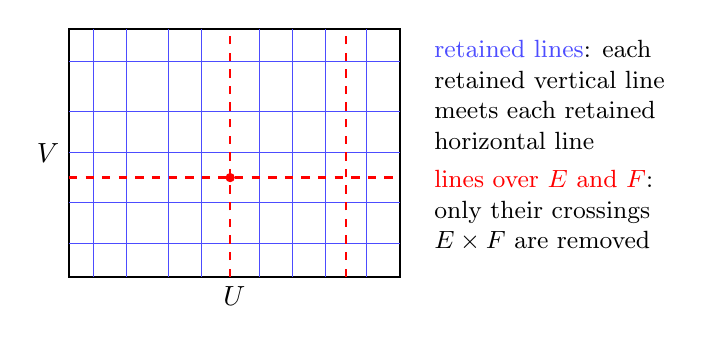
\begin{tikzpicture}[scale=1.05]
\draw[thick] (0,0) rectangle (4,3);
\foreach \x in {0.3,0.7,1.2,1.6,2.3,2.7,3.1,3.6} \draw[blue!70] (\x,0)--(\x,3);
\foreach \y in {0.4,0.9,1.5,2.0,2.6} \draw[blue!70] (0,\y)--(4,\y);
\foreach \x in {1.95,3.35} \draw[red,dashed,thick] (\x,0)--(\x,3);
\foreach \y in {1.2} \draw[red,dashed,thick] (0,\y)--(4,\y);
\fill[red] (1.95,1.2) circle (1.6pt);
\node[below] at (2,0) {$U$}; \node[left] at (0,1.5) {$V$};
\node[right,font=\small,align=left] at (4.3,2.2) {\textcolor{blue!70}{retained lines}: each\\ retained vertical line\\ meets each retained\\ horizontal line};
\node[right,font=\small,align=left] at (4.3,0.8) {\textcolor{red}{lines over $E$ and $F$}:\\ only their crossings\\ $E\times F$ are removed};
\end{tikzpicture}
\caption{The grid $G$ of Lemma~\ref{lem:grid}. Removing the meagre product $E\times F$ cannot disconnect the square.}\label{fig:grid}
\end{figure}

\subsection{Results quoted from the literature}
Only the following external results are used. Everything else is proved here.
\begin{center}
\small
\begin{tabular}{@{}p{0.48\textwidth}p{0.22\textwidth}p{0.2\textwidth}@{}}
\toprule
Statement & Source & Used in\\
\midrule
Local connectedness iff components of open sets are open & \cite[Theorem~25.3]{Mun00} & Prop.~\ref{prop:lc}, \ref{D4}\\
Boundary bumping (for an arbitrary nonempty proper subset) & \cite[Theorem~5.6]{Nad92} & Prop.~\ref{prop:lc}\\
Connected subsets of dendrites are arcwise connected & \cite[Proposition~10.9]{Nad92} & \ref{D1}\\
Intersections of connected subsets of dendrites are connected & \cite[Theorem~10.10]{Nad92} & \ref{D2}\\
Subcontinua of dendrites are dendrites & \cite[Corollary~10.6]{Nad92} & Lemma~\ref{lem:treestructure}\\
Locally connected continua without triods are arcs or circles & \cite[Theorem~75]{Moo62} & Fact~\ref{fact:notriod}\\
\bottomrule
\end{tabular}
\end{center}

% =====================================================================
\section{Reduction to dendrites}\label{sec:dendrite}

\begin{proposition}[Finite midsets force local connectedness; Loveland--Wayment {\cite[Lemma~2]{LW74}}]\label{prop:lc}
Let $(X,d)$ be a continuum in which $\M(a,b)$ is finite for all distinct $a,b$. Then $X$ is locally connected.
\end{proposition}

\begin{role}
This is the only place where the topology of $X$ is controlled directly. Without it a counterexample could be a wild continuum such as the topologist's sine curve. The proof below is self-contained apart from two textbook theorems. The result is due to Loveland and Wayment \cite[Lemma~2]{LW74}; its extension to Apollonius sets \cite[Lemma~2.2]{L76b} refers to that paper for the case of midsets.
\end{role}

\begin{proof}
Suppose $X$ is not locally connected. By \cite[Theorem~25.3]{Mun00} there are an open set $W$ and a component $Q$ of $W$ that is not open, so some $p\in Q$ is not an interior point of $Q$. Choose $\varepsilon>0$ with $B(p,\varepsilon)\subset W$ and with $U:=B(p,\varepsilon)\ne X$. This is possible since $X$ is nondegenerate. Let $C$ be the component of $U$ containing $p$. It is a connected subset of $W$ containing $p$, so $C\subset Q$. Hence no ball $B(p,\delta)$ is contained in $C$. So there are points $p_n\in U\setminus C$ with $p_n\to p$. Let $C_n$ be the component of $U$ containing $p_n$.

A component $C'\neq C$ of $U$ contains only finitely many $p_n$. Otherwise $p$ would lie in the closure of $C'$ in $U$; components of $U$ are closed in $U$, so $p\in C'$, and then $C'=C$. Passing to a subsequence, we may assume the $C_n$ are distinct, hence pairwise disjoint.

Put $E=X\setminus U$. It is nonempty because $U\ne X$, and proper because $p\in U$. Its complement is $X\setminus E=U$, so each $C_n$ is a component of $X\setminus E$. The boundary bumping theorem \cite[Theorem~5.6]{Nad92} gives $\cl(C_n)\cap\partial E\ne\emptyset$. Now $\partial E=\partial U=\cl U\setminus U$, because $U$ is open, and $\cl U\subset\{y:d(p,y)\le\varepsilon\}$ while $U=\{y:d(p,y)<\varepsilon\}$; hence $\partial E\subset\{y:d(p,y)=\varepsilon\}$. So there is $q_n\in\cl(C_n)$ with $d(p,q_n)=\varepsilon$. Pass to a subsequence with $q_n\to q$. Then $d(p,q)=\varepsilon$, so $q\ne p$.

Let $f=f_{p,q}$. It is $2$-Lipschitz, with $f(p)=-\varepsilon$ and $f(q)=\varepsilon$, so $f<0$ on $B(p,\varepsilon/4)$ and $f>0$ on $B(q,\varepsilon/4)$. For all large $n$ we have $p_n\in B(p,\varepsilon/4)$, and $C_n$ contains a point of $B(q,\varepsilon/4)$ because $q_n\in\cl(C_n)$ is close to $q$. By the intermediate value principle the connected set $C_n$ meets $\M(p,q)$. The $C_n$ are pairwise disjoint, so $\M(p,q)$ is infinite, a contradiction.
\end{proof}

\begin{figure}[ht]
\centering
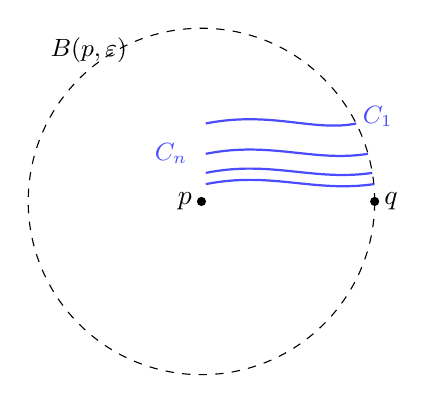
\begin{tikzpicture}[scale=1.1]
\draw[dashed] (0,0) circle (2);
\fill (0,0) circle (1.5pt) node[left] {$p$};
\fill (2,0) circle (1.5pt) node[right] {$q$};
\foreach \y/\n in {0.9/1,0.55/2,0.33/3,0.2/4}
  \draw[blue!70,thick] (0.05,\y) .. controls (0.8,\y+0.15) and (1.3,\y-0.1) .. ({sqrt(4-\y*\y)},\y);
\node[blue!70,right] at (1.75,0.98) {\small $C_1$};
\node[blue!70] at (-0.35,0.55) {\small $C_n$};
\node at (-1.3,1.75) {\small $B(p,\varepsilon)$};
\end{tikzpicture}
\caption{Proof of Proposition~\ref{prop:lc}. Disjoint components $C_n$ of the ball accumulate at $p$ and reach the sphere near $q$. Each contains a point equidistant from $p$ and $q$.}\label{fig:lc}
\end{figure}

\begin{proposition}[Simple closed curves]\label{prop:circle}
Let $(X,d)$ be a continuum with $|\M(a,b)|\le2$ for all distinct $a,b$. If $X$ contains a simple closed curve $C$, then $X=C$.
\end{proposition}
\begin{proof}
Suppose $z\in X\setminus C$. The continuous function $h_z|_C$ cannot be injective on a circle, so there are distinct $a,b\in C$ with $h_z(a)=h_z(b)$, that is, $z\in\M(a,b)$. The points $a,b$ divide $C$ into two arcs from $a$ to $b$. By the intermediate value principle each arc contains a point of $\M(a,b)$ other than $a$ and $b$. These two points and $z$ are three distinct points of $\M(a,b)$.
\end{proof}

\begin{remark}
Under the DMP, Proposition~\ref{prop:circle} is a special case of the theorem of Loveland and Wayment that a continuum with the DMP containing a nondegenerate subcontinuum without cut points is a simple closed curve \cite{LW74}; see \cite[Theorem~6(a)]{H01}. We include the short proof, which uses only the upper bound, to keep the argument self-contained.
\end{remark}

\begin{corollary}\label{cor:dendrite}
A continuum with the DMP is either a simple closed curve or a dendrite.
\end{corollary}
\begin{proof}
It is locally connected by Proposition~\ref{prop:lc}. If it contains a simple closed curve, it is one by Proposition~\ref{prop:circle}. Otherwise it is a dendrite by definition.
\end{proof}

% =====================================================================
\section{Branch points under the upper bound}\label{sec:branch}

\begin{convention}\label{conv:upper}
In this section $(X,d)$ is a dendrite with $|\M(a,b)|\le2$ for all distinct $a,b\in X$.
\end{convention}

We first record how to find disjoint ``test arms'' at a point.

\begin{lemma}[Arms]\label{lem:arms}
Let $c\in X$ have order at least $k$, where $k$ is finite, and let $K\subset X\setminus\{c\}$ be compact. Then there are arcs $B_1,\dots,B_k$, each having $c$ as an end, such that the sets $B_i\setminus\{c\}$ lie in distinct components of $X\setminus\{c\}$ (so the arcs pairwise meet only at $c$), with each $B_i$ disjoint from $K$ and of arbitrarily small diameter. If $f$ is a continuous function with $f(c)=0$ and finitely many zeros, the arms can be chosen so that $f$ has a constant strict sign on each $B_i\setminus\{c\}$.
\end{lemma}
\begin{proof}
Pick points $y_i$ in $k$ distinct components $C_i$ of $X\setminus\{c\}$. The set $[c,y_i]\setminus\{c\}$ is connected and contains $y_i$, so it lies in $C_i$. Replace $[c,y_i]$ by a short initial subarc from $c$ avoiding $K$ (possible since $d(c,K)>0$) and the finitely many zeros of $f$ other than $c$. The punctured arms are connected and carry no zero, so they have constant strict signs.
\end{proof}

The next lemma is the basic perturbation tool. Its first-hit variant goes back to Loveland \cite[Lemma~2.5]{L76b}, who worked under a continuity hypothesis. Here no continuity is needed; Figure~\ref{fig:radial} shows the idea.

\begin{lemma}[Radial monotonicity]\label{lem:radial}
Let $c$ be a branch point of $X$ and let $A$ be an arc having $c$ as an end, parametrized by $\alpha:[0,1]\to A$ with $\alpha(0)=c$. Then $h_c\circ\alpha$ is nondecreasing.
\end{lemma}

\begin{role}
Distances from a branch point never decrease as one moves away from it. This is used to bound the number of branch points (Theorem~\ref{thm:branchcount}), to locate centers of spheres (Lemma~\ref{lem:ownedge}), to count tips (Lemma~\ref{lem:pairs}), and in the triod (Theorem~\ref{thm:triod}).
\end{role}

\begin{proof}
Write $g=h_c\circ\alpha$, so $g(0)=0$. Suppose $0<\sigma<\tau\le1$ and $g(\sigma)>g(\tau)$. By Lemma~\ref{lem:extrema}(i) choose $\lambda\in(g(\tau),g(\sigma))$ (note $g(\tau)>0$, since $\alpha(\tau)\ne c$) that is not a local extremum value of $g$ on $(0,1)$. By the intermediate value theorem there are $\alpha_1\in(0,\sigma)$ and $\beta_1\in(\sigma,\tau)$ with $g(\alpha_1)=g(\beta_1)=\lambda$. Put $a=\alpha(\alpha_1)$ and $b=\alpha(\beta_1)$, and $f=f_{a,b}$. Then $f(c)=h_c(a)-h_c(b)=0$, and $c\notin[a,b]=\alpha([\alpha_1,\beta_1])$.

By Lemma~\ref{lem:arms} with $K=[a,b]$ take three arms at $c$, disjoint from $[a,b]$, on which $f$ has constant strict signs. Two of them, say $B_1,B_2$, carry the same sign $\eta\in\{\pm1\}$; fix test points $t_i\in B_i\setminus\{c\}$. By Lemma~\ref{lem:extrema}(iii) there are parameters $\alpha'$ arbitrarily close to $\alpha_1$ with $\eta\,(g(\alpha')-\lambda)<0$. Put $a'=\alpha(\alpha')$. By Lemma~\ref{lem:count}(a), if $\alpha'$ is close enough to $\alpha_1$ the strict signs at the test points $t_1,t_2,a,b$ survive, while the sign at $c$ is reversed on purpose:
\begin{center}
\small
\begin{tabular}{@{}lccccc@{}}
\toprule
 & at $c$ & at $t_1$ & at $t_2$ & at $a$ & at $b$\\
\midrule
$f_{a,b}$ & $0$ & $\eta$ & $\eta$ & $-$ & $+$\\
$f_{a',b}$ & $-\eta$ & $\eta$ & $\eta$ & $-$ & $+$\\
\bottomrule
\end{tabular}
\end{center}
The entries at $a$ and $b$ in the second row are $f_{a',b}(a)=d(a,a')-d(a,b)<0$ and $f_{a',b}(b)=d(b,a')>0$. By the second row, each of the arcs $[c,t_1]\subset B_1$, $[c,t_2]\subset B_2$ and $[a,b]$ contains points of both signs of $f_{a',b}$. The first two meet only at $c$, where $f_{a',b}\ne0$, because $B_1\setminus\{c\}$ and $B_2\setminus\{c\}$ lie in different components of $X\setminus\{c\}$; and both miss $[a,b]$. Lemma~\ref{lem:count}(b) gives $|\M(a',b)|\ge3$, a contradiction.
\end{proof}

\begin{figure}[ht]
\centering
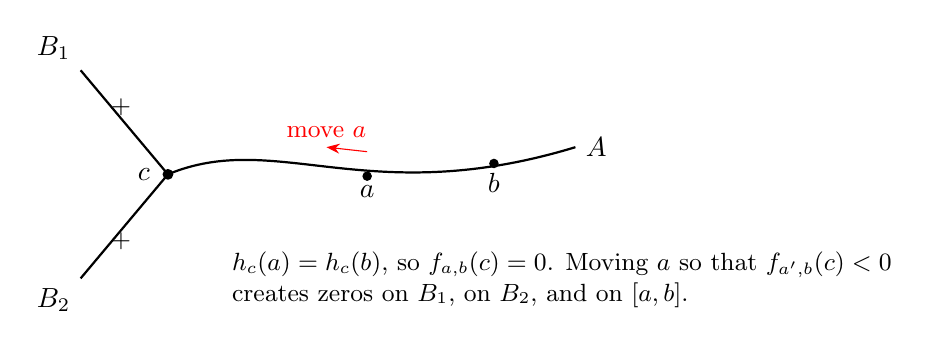
\begin{tikzpicture}[scale=1.15,>=Stealth]
\fill (0,0) circle (1.7pt) node[left=3pt] {$c$};
\draw[thick] (0,0)--(130:1.5) node[above left]{$B_1$};
\draw[thick] (0,0)--(230:1.5) node[below left]{$B_2$};
\node at (125:0.9) {\small $+$};
\node at (235:0.9) {\small $+$};
\draw[thick] (0,0) .. controls (1.2,0.5) and (2.2,-0.4) .. (4.5,0.3) node[right]{$A$};
\fill (2.2,-0.02) circle (1.5pt) node[below]{$a$};
\fill (3.6,0.12) circle (1.5pt) node[below]{$b$};
\draw[->,red] (2.2,0.25) -- (1.75,0.30) node[above,font=\small]{move $a$};
\node[font=\small,align=left,anchor=north west] at (0.6,-0.75) {$h_c(a)=h_c(b)$, so $f_{a,b}(c)=0$. Moving $a$ so that $f_{a',b}(c)<0$\\ creates zeros on $B_1$, on $B_2$, and on $[a,b]$.};
\end{tikzpicture}
\caption{Lemma~\ref{lem:radial}. If $h_c$ decreased along $A$, two sites at the same distance from $c$ could be perturbed to produce three equidistant points. Schematic: lengths and angles carry no metric meaning.}\label{fig:radial}
\end{figure}

\begin{lemma}[Order at most four]\label{lem:order}
Every point of $X$ has order at most four.
\end{lemma}
\begin{proof}
Suppose $c$ has order at least five, and take five arms $B_1,\dots,B_5$ at $c$ (Lemma~\ref{lem:arms}). Fix $\rho>0$ smaller than $h_c$ at the far end of each arm. Let $a\in B_1$ and $b\in B_2$ be the \emph{first} points, moving away from $c$, with $h_c=\rho$; so $h_c<\rho$ on $[c,a)$ and on $[c,b)$. Put $f=f_{a,b}$; then $f(c)=0$. Shorten all arms (Lemma~\ref{lem:arms}) so that $f$ has a constant strict sign on each punctured arm and the shortened $B_1,B_2$ end before $a,b$. Three arms carry the same sign $\eta$, and we fix a test point on each.

If $\eta=+1$, move $a$ to a point $a'\in[c,a)$ on the original arc close to $a$. Then $f_{a',b}(c)=h_c(a')-\rho<0$, while the three test signs persist by Lemma~\ref{lem:count}(a). If $\eta=-1$, move $b$ inward instead, so that $f_{a,b'}(c)=\rho-h_c(b')>0$. Either way, for the three arms with sign $\eta$ and their test points $t_i$, each arc $[c,t_i]$ carries both signs of the perturbed function; these arcs meet only at $c$, which is not a zero. Lemma~\ref{lem:count}(b) gives three zeros, a contradiction.
\end{proof}

\begin{theorem}[Few branch points]\label{thm:branchcount}
Suppose $X$ has a branch point $v$, of order $m$, and let $B$ be the set of branch points. Then $(m-2)(|B|-1)\le m$. In particular $|B|\le4$.
\end{theorem}

\begin{role}
Together with Corollary~\ref{cor:finitetree} this reduces the problem from arbitrary dendrites to finite trees. Only finite trees admit the finite parity count of Section~\ref{sec:signs}.
\end{role}

\begin{proof}
By Lemma~\ref{lem:order}, $m\in\{3,4\}$. Let $C_1,\dots,C_m$ be the components of $X\setminus\{v\}$, and fix once and for all a nondegenerate arc $I_j\subset C_j\cup\{v\}$ with end $v$, for each $j$.

Let $c\in B\setminus\{v\}$, say $c\in C_k$. For $j\ne k$ the set $[c,v]\cup I_j$ is an arc having $c$ as an end, because $[c,v]\setminus\{v\}\subset C_k$ and $I_j\setminus\{v\}\subset C_j$. By Lemma~\ref{lem:radial}, $h_c$ is nondecreasing along $I_j$ away from $v$, and in particular $h_c\ge h_c(v)$ on $I_j$.

\emph{Claim: $h_c$ is constant on $I_j$ for all $j\ne k$ with at most one exception.} Suppose $h_c$ is nonconstant on $I_j$ and on $I_l$, with $j\ne l$ and $j,l\ne k$. Then its maxima $\mu_j,\mu_l$ on these arcs exceed $h_c(v)$. By Lemma~\ref{lem:extrema}(i) choose $\lambda\in(h_c(v),\min\{\mu_j,\mu_l\})$ that is not a local extremum value of $h_c$ on either arc, and pick $a\in I_j$, $b\in I_l$ with $h_c(a)=h_c(b)=\lambda$. The arc $[a,b]=[a,v]\cup[v,b]$ lies in $I_j\cup I_l$ and misses $c$. Since $f_{a,b}(c)=0$, we argue as in the proof of Lemma~\ref{lem:radial}. Take three arms at $c$ disjoint from $[a,b]$ on which $f_{a,b}$ has constant strict signs (Lemma~\ref{lem:arms}); two of them carry the same sign $\eta$. By Lemma~\ref{lem:extrema}(iii) there are points $a'\in I_j$ arbitrarily close to $a$ with $\eta\,(h_c(a')-\lambda)<0$. Here we use that $a$ is not a local extremum of $h_c$ on $I_j$, by the choice of $\lambda$. For such $a'$ close to $a$, the sign table in the proof of Lemma~\ref{lem:radial} holds verbatim: the two test signs on the arms persist, $f_{a',b}$ still changes sign on $[a,b]$, and $\eta f_{a',b}(c)<0$. Lemma~\ref{lem:count}(b), applied exactly as there, gives three zeros of $f_{a',b}$. This proves the claim.

So for each $c\in B\setminus\{v\}$, the function $h_c$ is constant, equal to $d(c,v)>0$, on at least $m-2$ of the arcs $I_j$. No arc $I_j$ carries two such constant functions $h_c,h_{c'}$ with $c\ne c'$. Indeed, both would lie outside $I_j$, since their distances to it are positive. For distinct interior points $p,q$ of $I_j$, the midset $\M(p,q)$ would then contain $c$, $c'$ and a point of $(p,q)$. Counting incidences between any finite set $F\subset B\setminus\{v\}$ and the $m$ arcs gives $(m-2)|F|\le m$. Hence $|B\setminus\{v\}|\le m/(m-2)$, which is $3$ for $m=3$ and $2$ for $m=4$.
\end{proof}

\begin{corollary}\label{cor:finitetree}
A dendrite $X$ as in Convention~\ref{conv:upper} is a finite tree.
\end{corollary}
\begin{proof}
If $X$ has no branch point, it is an arc by Fact~\ref{fact:notriod}. Otherwise, by Theorem~\ref{thm:branchcount} and Lemma~\ref{lem:order}, $X$ has finitely many branch points, each of finite order. In both cases $X$ is a finite tree in the sense of Definition~\ref{def:tree}, with the structure described in Lemma~\ref{lem:treestructure}.
\end{proof}

% =====================================================================
\section{Signs on a finite tree}\label{sec:signs}

\begin{convention}[Standing assumption for Sections~\ref{sec:signs}--\ref{sec:arc}]\label{conv:tree}
$T$ is a finite tree with a compatible metric $d$ having the DMP, with vertex set $\Ver$, odd-degree vertices $\Odd$, and the terminology of Definition~\ref{def:tree}. Since $T$ is a dendrite with $|\M|\le2$, the results of Section~\ref{sec:branch} apply. A tree is \emph{branched} if it has a branch point.
\end{convention}

For the reader's convenience we collect the notation used from here on.
\begin{center}
\small
\begin{tabular}{@{}p{0.27\textwidth}p{0.66\textwidth}@{}}
\toprule
Notation & Meaning\\
\midrule
$h_x=d(x,\cdot)$ & distance seen by the observer $x$\\
$f_{a,b}=h_\cdot(a)-h_\cdot(b)$ & sign function of the sites $a,b$; negative at $a$, positive at $b$\\
$\M(a,b)$, $S(x,r)$ & midset $f_{a,b}^{-1}(0)$; metric sphere\\
$\Ver$, $\Odd$, tip & vertices (tips and branch points); odd-degree vertices; point of order one\\
edge $\ell$, open edge $\ell^\circ$ & arc between adjacent vertices; the edge minus its two ends\\
edge point & point of $T\setminus\Ver$ (order two)\\
strict pair, $\N(a,b)$ & no vertex in $\M(a,b)$; number of odd-degree vertices closer to $a$\\
crossing, touch & zero in an open edge with / without a sign change\\
spherical arc, center & nondegenerate arc in $S(x,r)$, $r>0$; the point $x$\\
box, odd box & $U\times V$ of disjoint open arcs in open edges; all pairs strict with $\N$ odd\\
\bottomrule
\end{tabular}
\end{center}

\begin{definition}[Strict pairs and the count $\N$]\label{def:strict}
A pair of distinct sites $(a,b)$ is \emph{strict} if $f_{a,b}(u)\ne0$ for every vertex $u\in\Ver$, that is, if no vertex is equidistant from $a$ and $b$. For a strict pair put
\[
  \N(a,b)=\bigl|\{u\in\Odd:\ f_{a,b}(u)<0\}\bigr| = \bigl|\{u\in\Odd:\ d(u,a)<d(u,b)\}\bigr|.
\]
\end{definition}

\noindent
Thus $\N(a,b)$ counts the odd-degree vertices that are closer to $a$. We use this sign convention throughout: for $u\in\Odd$ and a strict pair $(a,b)$,
\begin{equation}\label{eq:signconv}
  f_{a,b}(u)<0\iff h_u(a)<h_u(b)\iff u\ \text{is counted in}\ \N(a,b).
\end{equation}
In words, when the first site is moved to the second, the vertices counted are those whose distance \emph{increases}. Strictness is an open condition on pairs, and $\N$ is locally constant on strict pairs, by \eqref{eq:lip}. Since $f_{b,a}=-f_{a,b}$ and $|\Odd|$ is even,
\begin{equation}\label{eq:swap}
  \N(b,a)=|\Odd|-\N(a,b)\equiv \N(a,b)\pmod 2 .
\end{equation}

\begin{definition}[Crossings and touches]\label{def:crossing}
Let $g:T\to\mathbb R$ be continuous with finitely many zeros, and let $y$ be a zero that is an edge point. Take a small open arc $J\ni y$ in its open edge with $J\cap g^{-1}(0)=\{y\}$; the two components of $J\setminus\{y\}$ are the two \emph{sides} of $y$. Then $y$ is a \emph{crossing} if $g$ has opposite signs on the two sides, and a \emph{touch} if the signs agree (Figure~\ref{fig:crosstouch}).
\end{definition}

\begin{figure}[ht]
\centering
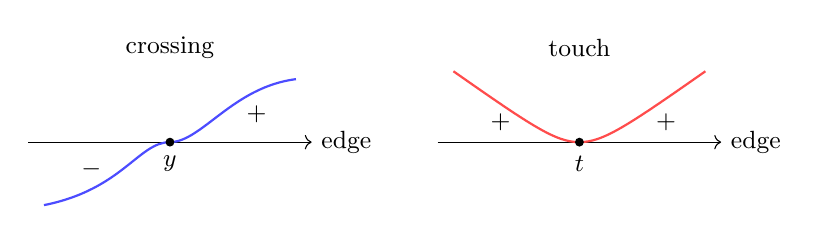
\begin{tikzpicture}[scale=1.0]
\begin{scope}
\draw[->] (-0.2,0)--(3.4,0) node[right]{\small edge};
\draw[thick,blue!70] (0,-0.8) .. controls (1,-0.6) and (1.2,0) .. (1.6,0) .. controls (2,0) and (2.4,0.7) .. (3.2,0.8);
\fill (1.6,0) circle (1.6pt);
\node[below] at (1.6,-0.05) {\small $y$};
\node at (1.6,1.2) {\small crossing};
\node at (0.6,-0.35) {\small $-$}; \node at (2.7,0.35) {\small $+$};
\end{scope}
\begin{scope}[xshift=5.2cm]
\draw[->] (-0.2,0)--(3.4,0) node[right]{\small edge};
\draw[thick,red!70] (0,0.9) .. controls (1,0.2) and (1.3,0) .. (1.6,0) .. controls (1.9,0) and (2.2,0.2) .. (3.2,0.9);
\fill (1.6,0) circle (1.6pt);
\node[below] at (1.6,-0.05) {\small $t$};
\node at (1.6,1.2) {\small touch};
\node at (0.6,0.25) {\small $+$}; \node at (2.7,0.25) {\small $+$};
\end{scope}
\end{tikzpicture}
\caption{The graph of $g$ along an edge near a crossing $y$ and near a touch $t$. A touch can be pushed below the axis by an arbitrarily small change of $g$, producing two zeros.}\label{fig:crosstouch}
\end{figure}

\begin{lemma}[Parity]\label{lem:parity}
Let $T'$ be a finite tree with vertex set $\Ver'$ and odd-degree vertices $\Odd'$. Let $g:T'\to\mathbb R$ be continuous with finitely many zeros, none of them a vertex. Then
\[
  |\{\text{crossings of }g\}|\ \equiv\ |\{u\in\Odd':g(u)<0\}|\pmod 2 .
\]
\end{lemma}

\begin{role}
This is the only global, topological input on a tree. It turns the two-point condition into a dichotomy: a strict pair has either two crossings or a crossing and a touch (Corollary~\ref{cor:types}).
\end{role}

\begin{proof}
On an edge $\ell$ with ends $u,u'$ the sign of $g$ changes exactly at the crossings in the open edge $\ell^\circ$. Hence the number of crossings in $\ell^\circ$ is congruent modulo two to $[g(u)<0]+[g(u')<0]$, where $[\cdot]$ is $1$ for a true statement and $0$ otherwise. Summing over all edges, each vertex $u$ is counted $\deg u$ times, so the total is congruent to $\sum_{u}\deg(u)[g(u)<0]\equiv\sum_{u\in\Odd'}[g(u)<0]$.
\end{proof}

We apply this lemma to $T$ itself, and in Lemma~\ref{lem:tips} to a tree obtained from $T$ by cutting off a short end of a terminal edge.

\begin{corollary}[Two types of strict pairs]\label{cor:types}
Let $(a,b)$ be a strict pair. Then $\M(a,b)$ consists of two edge points. The arc $[a,b]$ contains an odd number of crossings, hence at least one. Moreover:
\begin{itemize}[nosep]
\item if $\N(a,b)$ is even, both points of $\M(a,b)$ are crossings;
\item if $\N(a,b)$ is odd, $\M(a,b)$ consists of one crossing and one touch.
\end{itemize}
\end{corollary}
\begin{proof}
No vertex is a zero, so both zeros are edge points. Along $[a,b]$, $f_{a,b}$ goes from negative to positive, so it changes sign an odd number of times. Each sign change occurs at a zero $y$ in the interior of $[a,b]$. Since $y$ has order two, $[a,b]$ coincides near $y$ with the open edge of $y$, so the sign changes along $[a,b]$ are exactly the crossings on $[a,b]$. The rest follows from Lemma~\ref{lem:parity} with $T'=T$ and $g=f_{a,b}$, since there are exactly two zeros.
\end{proof}

The second basic tool says that a touch cannot be moved off the axis in the wrong direction (Figure~\ref{fig:crosstouch}). This is the source of all the rigidity below. In Section~\ref{sec:spheres} it will show that the touch cannot drift as the sites move: the values it would sweep out are, apart from countably many exceptions, points from which both sites are local extrema of distance, and the set of such pairs is too small to separate the space of pairs.

\begin{lemma}[Stability of a touch]\label{lem:stability}
Let $(a,b)$ be a strict pair with $\N(a,b)$ odd, and let $t$ be the touch in $\M(a,b)$. If $a$ is an edge point, then $a$ is a local extremum of $h_t$ restricted to the open edge containing $a$. The same holds for $b$.
\end{lemma}

\begin{role}
This is where the exact count ``two'' enters most directly. It converts the topological type of a zero into metric information about the sites, and it feeds the Baire argument of Proposition~\ref{prop:oddbox}.
\end{role}

\begin{proof}
Let $y$ be the crossing, and let $\sigma\in\{\pm1\}$ be the common sign of $f_{a,b}$ on both sides of $t$. Choose test points $t_-,t_+$ on the two sides of $t$, and $y_-,y_+$ on the two sides of $y$, such that the arcs $[t_-,t_+]$ and $[y_-,y_+]$ are disjoint and contain no zero other than $t$ and $y$, respectively. Then $\sigma f_{a,b}(t_\pm)>0$ and $f_{a,b}(y_-)f_{a,b}(y_+)<0$. By \eqref{eq:lip} these four strict signs persist for $f_{a',b}$ when $a'$ is close to $a$.

If for such an $a'$ we had $\sigma f_{a',b}(t)<0$, then each of $[t_-,t]$, $[t,t_+]$ and $[y_-,y_+]$ would carry both signs of $f_{a',b}$. The first two meet only at $t$, where $f_{a',b}\ne0$, and both miss $[y_-,y_+]$, so Lemma~\ref{lem:count}(b) would give three zeros. Hence $\sigma f_{a',b}(t)\ge0$ for all $a'$ near $a$. Since $t\in\M(a,b)$, we have $f_{a',b}(t)=h_t(a')-h_t(b)=h_t(a')-h_t(a)$. Thus $a$ is a local minimum of $h_t$ if $\sigma=+1$ and a local maximum if $\sigma=-1$. For $b$, apply the same argument to $f_{a,b'}(t)=h_t(a)-h_t(b')=h_t(b)-h_t(b')$.
\end{proof}

% =====================================================================
\section{Spherical arcs and odd boxes}\label{sec:spheres}

\begin{definition}[Spherical arcs]\label{def:spherical}
A \emph{spherical arc} is a nondegenerate arc $I\subset T$ contained in a sphere $S(x,r)$ with $r>0$. The point $x$ is a \emph{center} of $I$ and $r$ its \emph{radius}. Note that $x\notin I$.
\end{definition}

Spherical arcs are the rigid objects that the touches will produce. The next lemma lists their basic properties.

\begin{lemma}[Spherical arcs]\label{lem:sphericalarc}
Let $I$ be a spherical arc with center $x$ and radius $r$.
\begin{enumerate}[label=\textup{(\alph*)}]
\item For every $y\notin I\cup\{x\}$, the function $h_y$ is strictly monotone on $I$.
\item The center is unique: for no point $x'\ne x$ is $h_{x'}$ constant on $I$. Every nondegenerate subarc of $I$ is spherical with the same center.
\item No point of $I$ other than its ends is a vertex. So the interior of $I$ consists of edge points, and $I$ lies in one edge.
\item The set of all points of $T$ that are centers of some spherical arc is countable.
\end{enumerate}
\end{lemma}
\begin{proof}
(a) If $h_y(p)=h_y(q)$ for distinct $p,q\in I$, then $\M(p,q)$ contains $x$ and $y$, and also a point of the arc $(p,q)\subset I$, which differs from both. That is three points.

(b) A second center $x'$ has positive radius (as $I$ is nondegenerate), so $x'\notin I$, and $h_{x'}$ is constant on $I$, contradicting (a). The second statement is clear.

(c) An interior point of an arc is not a tip, by Lemma~\ref{lem:separate}. Suppose a branch point $y$ were interior to $I$. The union of the edges at $y$ is a neighborhood of $y$ in $T$ (Lemma~\ref{lem:treestructure}), so near $y$ the arc $I$ runs along two of the edges at $y$; let $z_n\to y$ be points of the open edge of a third edge at $y$, with $z_n\ne x$. By Lemma~\ref{lem:separate}, $I\setminus\{y\}$ lies in the two components of $T\setminus\{y\}$ containing the other two edges, so $z_n\notin I$. Fix a closed subarc $I'\subset I$ having $y$ in its interior. By (a) each $h_{z_n}$ is strictly monotone on $I'$. After passing to a subsequence, all are increasing or all decreasing in a fixed orientation. Since $|h_{z_n}-h_y|\le d(z_n,y)\to0$ uniformly, $h_y$ is weakly monotone on $I'$. But $h_y(y)=0<h_y$ elsewhere on $I'$, so $h_y$ has a strict minimum at an interior point of $I'$. This is a contradiction.

(d) Identify each edge with $[0,1]$. Every spherical arc contains a nondegenerate subarc lying in one edge with rational parameter endpoints, and this subarc is spherical with the same center by (b). There are countably many such subarcs, and by (b) each has at most one center.
\end{proof}

The following lemma is the first consequence of Lemma~\ref{lem:stability}. It describes what happens when one site lies on a spherical arc and the other does not.

\begin{lemma}[Off-sphere parity]\label{lem:offsphere}
Let $I$ be a spherical arc with center $x$ and radius $r$, let $p$ be an interior point of $I$, and let $b\ne p$ satisfy $h_x(b)\ne r$. If $(p,b)$ is strict, then $\N(p,b)$ is even.
\end{lemma}

\begin{role}
This lemma is used repeatedly. It says that when one site lies on a spherical arc and the other is off its sphere, the pair cannot be strict with $\N$ odd. In the later arguments a parity flip at one vertex then forces the second site back onto the sphere.
\end{role}

\begin{proof}
Suppose $\N(p,b)$ is odd, and let $t$ be the touch in $\M(p,b)$ (Corollary~\ref{cor:types}). By Lemma~\ref{lem:sphericalarc}(c), $p$ is an edge point. By Lemma~\ref{lem:stability}, $p$ is a local extremum of $h_t$ on its edge. But $t\ne p$, since $f_{p,b}(p)<0$, and $t\ne x$, since $h_x(p)=r\ne h_x(b)$. Choose a closed subarc $I'\subset I$ containing $p$ in its interior and not containing $t$. By Lemma~\ref{lem:sphericalarc}(a), $h_t$ is strictly monotone on $I'$, so $p$ is not a local extremum. This is a contradiction.
\end{proof}

\begin{definition}[Boxes]\label{def:box}
A \emph{box} is a product $U\times V$ of two disjoint open arcs, each contained in an open edge (possibly the same open edge). A box is \emph{odd} if every pair $(a,b)\in U\times V$ is strict with $\N(a,b)$ odd.
\end{definition}

\noindent
Because strictness and $\N$ are locally constant, every strict pair $(a,b)$ of edge points with $\N(a,b)$ odd is contained in an odd box $U\times V$ with $a\in U$ and $b\in V$. The central result of this section is that an odd box always lies on a single sphere.

\begin{proposition}[Odd boxes lie on a sphere]\label{prop:oddbox}
Let $U\times V$ be an odd box. Then there are $c\in T$ and $r>0$ with $U\cup V\subset S(c,r)$. The point $c$ is unique.
\end{proposition}

\begin{role}
This is the main rigidity statement. Every later step obtains its contradictions by producing an odd box and then asking where the center $c$ can be. Lemmas~\ref{lem:tips} and \ref{lem:ownedge} rule out the obvious locations, and the boundary argument of Lemma~\ref{lem:boundary} rules out the rest.
\end{role}

The proof has five stages, which we label for later reference:
\begin{enumerate}[label=\textup{(S\arabic*)},leftmargin=*]
\item Baire category gives uniform separation of the two midset points on a smaller box.
\item Uniform separation gives Hausdorff continuity of the midset on that box.
\item A protected crossing identifies the other midset point, continuously, as the touch.
\item The connected grid forces the touch to be constant.
\item Off-sphere parity extends the resulting sphere to the whole original box.
\end{enumerate}
Lemma~\ref{lem:selection} below carries out (S1)--(S3); the proof of Proposition~\ref{prop:oddbox}, which follows it, carries out (S4)--(S5).

\begin{lemma}[Continuous selection of the touch]\label{lem:selection}
Let $U\times V$ be an odd box. There are a nonempty box $U_1\times V_1\subset U\times V$, an open arc $J$ in an open edge, and a continuous map $w:U_1\times V_1\to J$ such that $w(a,b)$ is the touch of $\M(a,b)$ for every $(a,b)\in U_1\times V_1$.
\end{lemma}

\begin{proof}
\emph{(S1) Uniform separation.} For $n\ge1$ let $A_n$ be the set of $(a,b)\in U\times V$ whose two midset points are at distance at least $1/n$. Each $A_n$ is relatively closed in $U\times V$. Indeed, let $(a_k,b_k)\to(a,b)$ in $U\times V$ with $\M(a_k,b_k)=\{y_k,z_k\}$ and $d(y_k,z_k)\ge1/n$. By compactness of $T$ we may assume $y_k\to y$ and $z_k\to z$. By \eqref{eq:lip}, $f_{a_k,b_k}\to f_{a,b}$ uniformly, so $y,z\in\M(a,b)$. Also $d(y,z)\ge1/n$, so $\{y,z\}=\M(a,b)$ and $(a,b)\in A_n$. The sets $A_n$ cover $U\times V$, because every midset has two distinct points. By the Baire category theorem some $A_n$ contains a nonempty box $W_0$.

\emph{(S2) Hausdorff continuity on $W_0$.} We claim: for every $(a,b)\in W_0$ and $\varepsilon>0$ there is $\delta>0$ such that, whenever $(a',b')\in W_0$ with $d(a,a')+d(b,b')<\delta$, each point of $\M(a',b')$ lies within $\varepsilon$ of a point of $\M(a,b)$ and each point of $\M(a,b)$ lies within $\varepsilon$ of a point of $\M(a',b')$. If not, there are $(a_k,b_k)\to(a,b)$ in $W_0$ for which this fails. Write $\M(a_k,b_k)=\{y_k,z_k\}$, with $d(y_k,z_k)\ge1/n$ since $(a_k,b_k)\in W_0$. Passing to a subsequence, $y_k\to y$ and $z_k\to z$; as in (S1), $\{y,z\}=\M(a,b)$. Then for large $k$ the point $y_k$ is within $\varepsilon$ of $y$ and $z_k$ is within $\varepsilon$ of $z$, so the property holds for these $k$, a contradiction.

This continuity is local. Without uniform separation the two points of $\M(a_k,b_k)$ might converge to a single point of $\M(a,b)$, leaving its other point unapproximated; this is why (S1) comes first. No continuity of the midset map on all pairs is claimed or used.

\emph{(S3) The touch label.} Fix $(\bar a,\bar b)\in W_0$ with crossing $y_0$ and touch $t_0$ (Corollary~\ref{cor:types}). Choose open arcs $J_y\ni y_0$ and $J\ni t_0$ inside open edges, with disjoint closures. Choose test points $y_\pm\in J_y$ on the two sides of $y_0$ with $f_{\bar a,\bar b}(y_-)f_{\bar a,\bar b}(y_+)<0$, such that $y_0$ is the only zero on $[y_-,y_+]$; this \emph{protects} the crossing. Take $\varepsilon>0$ so small that the $\varepsilon$-ball about $y_0$ lies in $(y_-,y_+)$ and the $\varepsilon$-ball about $t_0$ lies in $J$. By (S2) and \eqref{eq:lip} there is a box $U_1\times V_1\subset W_0$ around $(\bar a,\bar b)$ on which: the signs at $y_\pm$ persist; and $\M(a,b)$ has one point within $\varepsilon$ of $y_0$ and one within $\varepsilon$ of $t_0$. So $\M(a,b)$ has exactly one point $\gamma(a,b)\in(y_-,y_+)$ and exactly one point $w(a,b)\in J$. Since $f_{a,b}$ has opposite signs at $y_\pm$ and a single zero between them, $\gamma(a,b)$ is a crossing. By Corollary~\ref{cor:types} the other point $w(a,b)$ is the touch. Finally, $w$ is continuous. Let $(a_k,b_k)\to(a,b)$ in $U_1\times V_1$, and let $0<\varepsilon'<d\bigl(w(a,b),\cl J_y\bigr)$. By (S2), for large $k$ some point of $\M(a_k,b_k)$ lies within $\varepsilon'$ of $w(a,b)$. It is not $\gamma(a_k,b_k)\in J_y$, so it is $w(a_k,b_k)$. Hence $w(a_k,b_k)\to w(a,b)$.
\end{proof}

\begin{proof}[Proof of Proposition~\ref{prop:oddbox}]
Take $U_1\times V_1$, $J$ and $w$ from Lemma~\ref{lem:selection}, and identify $J$ with an open interval via a homeomorphism $\varphi$.

\emph{(S4) The touch is constant.} Suppose $w$ is not constant on $U_1\times V_1$. Its image is connected, so $\varphi\circ w$ has an interval of values with nonempty interior. That interior is uncountable, while by Lemma~\ref{lem:sphericalarc}(d) only countably many points are centers of spherical arcs. So we can choose $z$ in the image with $\varphi(z)$ interior to $\varphi(w(U_1\times V_1))$ such that $z$ is not the center of any spherical arc. Then $h_z$ is constant on no nondegenerate arc. By Lemma~\ref{lem:extrema}(ii), the sets $E\subset U_1$ and $F\subset V_1$ of local extrema of $h_z|_{U_1}$ and of $h_z|_{V_1}$ are meagre. By Lemma~\ref{lem:stability}, $w(a,b)=z$ implies that $a\in E$ and $b\in F$, so
\[
  w^{-1}(z)\subset E\times F .
\]
Hence $g=\varphi\circ w-\varphi(z)$ has no zero on $(U_1\times V_1)\setminus(E\times F)$, which is exactly the grid $G$ of Lemma~\ref{lem:grid}. That lemma shows that $g\ge0$ everywhere or $g\le0$ everywhere, so $\varphi(z)$ is an endpoint of the interval $\varphi(w(U_1\times V_1))$. This contradicts the choice of $z$. Hence $w\equiv c$ for some $c\in J$.

Meagreness alone would not suffice here. A meagre subset of a square can disconnect it; a single vertical segment does. The decisive point is that $w^{-1}(z)$ lies in a \emph{product} of meagre sets, whose complement is connected by Lemma~\ref{lem:grid}.

\emph{A sphere on the subbox.} For all $a\in U_1$ and $b\in V_1$ we have $h_c(a)=h_c(b)$. Fixing $b$ shows that $h_c$ is constant on $U_1$; fixing $a$ shows it is constant on $V_1$, with the same value $r$. If $r=0$ then $U_1\subset\{c\}$, which is absurd. So $U_1\cup V_1\subset S(c,r)$ with $r>0$.

\emph{(S5) Extension to the whole box.} Fix $a_1\in U_1$; it is an interior point of a spherical arc contained in $U_1$. Let $b\in V$. The pair $(a_1,b)$ is strict with $\N(a_1,b)$ odd. If $h_c(b)\ne r$, Lemma~\ref{lem:offsphere} would make $\N(a_1,b)$ even. Hence $V\subset S(c,r)$. Now fix $b_1\in V$, an interior point of a spherical arc in $V$, and let $a\in U$. By \eqref{eq:swap}, $\N(b_1,a)$ is odd, so the same argument with the roles of the sites exchanged gives $h_c(a)=r$. Uniqueness of $c$ follows from Lemma~\ref{lem:sphericalarc}(b).
\end{proof}

\begin{corollary}\label{cor:oddpair}
Let $(a,b)$ be a strict pair of edge points with $\N(a,b)$ odd. Then there are a unique $c\in T$, a radius $r>0$, and open arcs $U\ni a$ and $V\ni b$ in open edges with $U\cup V\subset S(c,r)$. Moreover $c\in\M(a',b')$ for all $(a',b')\in U\times V$; in particular $c$ is an edge point.
\end{corollary}
\begin{proof}
Apply Proposition~\ref{prop:oddbox} to an odd box $U\times V$ around $(a,b)$. For $(a',b')\in U\times V$ we have $h_c(a')=r=h_c(b')$, so $c\in\M(a',b')$. Since $(a',b')$ is strict, $c$ is not a vertex.
\end{proof}

\subsection*{What remains}
Proposition~\ref{prop:oddbox} attaches to every odd box a forced center $c$. The remaining sections pursue a single question: \emph{where can this center lie?} Section~\ref{sec:centers} shows that the center of a spherical arc is never a tip and never lies in the open edge carrying the arc. Section~\ref{sec:tips} follows a family of odd pairs to the boundary of the region where they are odd. There the forced center becomes a midset point of a boundary pair, and the two candidates for it are exactly the locations excluded in Section~\ref{sec:centers}. This yields strict monotonicity of distances to the tips, which Sections~\ref{sec:count}--\ref{sec:triod} turn into a counting contradiction. Section~\ref{sec:arc} treats the arc by a separate matching argument.

% =====================================================================
\section{Where the center of a spherical arc can lie}\label{sec:centers}

We now show that centers of spherical arcs avoid two kinds of location: tips, and the open edge containing the arc. Throughout, Convention~\ref{conv:tree} is in force.

\begin{lemma}[Tips are not centers]\label{lem:tips}
No tip of $T$ is the center of a spherical arc.
\end{lemma}

\begin{role}
Used in Proposition~\ref{prop:tipdistance}(a) to show that the distance from a tip is constant on no arc. It holds for every finite tree with the DMP, including the arc. For centers of odd boxes, the conclusion is immediate from Corollary~\ref{cor:oddpair}; the point of the lemma is that it applies to every spherical arc.
\end{role}

\begin{proof}
Let $x$ be a tip and $I$ a spherical arc with center $x$ and radius $r$. By Lemma~\ref{lem:sphericalarc}(b),(c) we may shrink $I$ so that it lies in an open edge. Fix $i\in I$ and let $s$ be the last point of the arc $[i,x]$ lying in $I$; it exists because $[i,x]\cap I$ is compact. Then $[s,x]\cap I=\{s\}$, and $s$ is an end of $I$. Indeed, an interior point of $I$ is an edge point, so it has a neighborhood in $T$ that is an open arc contained in $I$; the arc $[s,x]$ starts at $s$, so it would contain further points of $I$. On the arc $[s,x]$ let $q$ be the point closest to $x$ with $h_x(q)=r$. It exists because the set is closed and contains $s$, and $q\ne x$ because $h_x(x)=0$. Then $h_x<r$ on $(q,x]$, by the intermediate value theorem and the choice of $q$. See Figure~\ref{fig:tip}.

Every vertex $u\ne x$ lies outside $I\cup\{x\}$. By Lemma~\ref{lem:sphericalarc}(a), $h_u$ takes the value $h_u(q)$ at most once on $I$. So we can choose an interior point $p$ of $I$ with
\[
  h_u(p)\ne h_u(q)\qquad\text{for all } u\in\Ver\setminus\{x\}.
\]
Then $\M(p,q)$ contains $x$, since $h_x(p)=r=h_x(q)$, and a point $y$ of the arc $(p,q)$. Note that $x\notin[p,q]=[p,s]\cup[s,q]$, because $x$ is the far end of $[s,x]$ and $q\ne x$. So $\M(p,q)=\{x,y\}$. The zero $y$ is not a vertex, by the choice of $p$, and it is the only zero on $[p,q]$, so it is a crossing. On $[q,x)$ there is no zero and $f_{p,q}(q)=d(p,q)>0$, so $f_{p,q}>0$ there.

Choose $x'\in(q,x)$ so close to $x$ that $(x',x]$ lies in the terminal edge of $x$, and let $T'=T\setminus(x',x]$. This is a finite tree in which the tip $x$ is replaced by the tip $x'$ and all other degrees are unchanged:
\[
  \Ver(T')=(\Ver\setminus\{x\})\cup\{x'\},\qquad \Odd(T')=(\Odd\setminus\{x\})\cup\{x'\},\qquad f_{p,q}(x')>0 .
\]
Since $x\notin T'$, the function $f_{p,q}|_{T'}$ has the single zero $y$, which is a crossing. Lemma~\ref{lem:parity} on $T'$ gives
\[
  |\{u\in\Odd\setminus\{x\}: f_{p,q}(u)<0\}|\ \text{ is odd.}
\]
Now take $b\in(q,x')$ close to $q$. By \eqref{eq:lip}, $f_{p,b}(u)$ has the same strict sign as $f_{p,q}(u)$ for $u\in\Ver\setminus\{x\}$. Also $f_{p,b}(x)=r-h_x(b)>0$. So $(p,b)$ is strict and $\N(p,b)$ is odd, while $h_x(b)<r$. This contradicts Lemma~\ref{lem:offsphere}.
\end{proof}

\begin{figure}[ht]
\centering
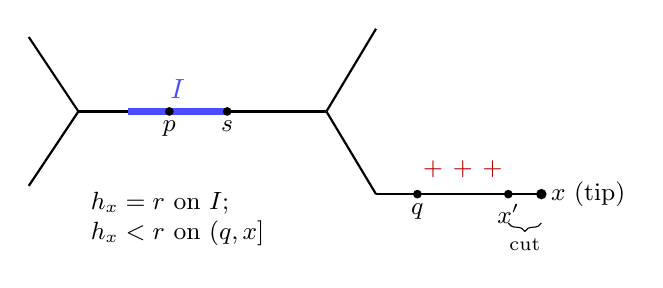
\begin{tikzpicture}[scale=1.05]
\draw[thick] (0,0)--(3,0);
\draw[thick] (3,0)--(3.6,1.0); \draw[thick] (3,0)--(3.6,-1.0);
\draw[thick] (-0.6,0.9)--(0,0)--(-0.6,-0.9);
\draw[line width=2.4pt,blue!70] (0.6,0)--(1.8,0) node[midway,above]{$I$};
\fill (1.8,0) circle (1.5pt) node[below]{\small $s$};
\fill (1.1,0) circle (1.5pt) node[below]{\small $p$};
\draw[thick] (3.6,-1.0)--(5.6,-1.0);
\fill (4.1,-1.0) circle (1.5pt) node[below]{\small $q$};
\fill (5.2,-1.0) circle (1.5pt) node[below]{\small $x'$};
\fill (5.6,-1.0) circle (1.8pt) node[right]{\small $x$ (tip)};
\node[font=\small,red!70!black] at (4.65,-0.7) {$+\,+\,+$};
\draw[decorate,decoration={brace,amplitude=3pt,mirror}] (5.2,-1.35)--(5.6,-1.35) node[midway,below=2pt,font=\scriptsize]{cut};
\node[font=\small,align=left] at (1.2,-1.3) {$h_x=r$ on $I$;\\ $h_x<r$ on $(q,x]$};
\end{tikzpicture}
\caption{Lemma~\ref{lem:tips}. Cutting off the positive end $(x',x]$ leaves one crossing. Parity then fixes the vertex signs, and a site $b$ just beyond $q$ contradicts Lemma~\ref{lem:offsphere}. Schematic: lengths carry no metric meaning.}\label{fig:tip}
\end{figure}

\begin{lemma}[The center is a crossing]\label{lem:crossing}
Let $x$ be an edge point and $r>0$, and let $K$ be a nondegenerate component of $S(x,r)$. Then $K$ is an arc contained in one edge; its ends may be vertices. For all distinct $p,q\in K$, the pair $(p,q)$ is strict, $\N(p,q)$ is even, and $\M(p,q)=\{x,y\}$ with $y\in(p,q)$, where both $x$ and $y$ are crossings.
\end{lemma}

\begin{role}
This lemma gives the parity of pairs inside a spherical arc and the sign pattern around its center. It is used in Lemma~\ref{lem:ownedge}, in the column argument of Theorem~\ref{thm:triod}, and in Theorem~\ref{thm:arc}.
\end{role}

\begin{proof}
$K$ is a closed connected subset of $T$. If it contained two points not lying in a common edge, the arc between them would lie in $K$ by \ref{D1}--\ref{D2}, would be spherical, and would contain a vertex in its interior, contrary to Lemma~\ref{lem:sphericalarc}(c). So $K$ is a closed subarc of one edge, and $x\notin K$.

Let $q_0$ be the end of $K$ through which the arc from $K$ to $x$ leaves $K$. Points of $[q_0,x]$ off the sphere accumulate at $q_0$. Otherwise some arc $[q_0,q']\subset[q_0,x]$ with $q'\ne q_0$ would lie in $S(x,r)$. Then $K\cup[q_0,q']$ would be connected, since the two sets share $q_0$, and contained in $S(x,r)$. It is strictly larger than $K$, because $[q_0,x]\cap K=\{q_0\}$. This contradicts the fact that $K$ is a component. Let $p$ be a point of $K$ other than its two ends. The midset $\M(p,q_0)$ contains $x$ and a point $y\in(p,q_0)$. Since $x\notin K\supset[p,q_0]$, we get $\M(p,q_0)=\{x,y\}$. Both are edge points, so $(p,q_0)$ is strict, and $y$, the only zero on $[p,q_0]$, is a crossing. Take $b_n\to q_0$ in $[q_0,x]$ with $h_x(b_n)\ne r$. For large $n$ the pair $(p,b_n)$ is strict with $\N(p,b_n)=\N(p,q_0)$. By Lemma~\ref{lem:offsphere} this number is even. By Corollary~\ref{cor:types} both zeros of $f_{p,q_0}$ are crossings; in particular $x$ is a crossing.

Now let $p',q'\in K$ be arbitrary and distinct. For each vertex $u$, $h_u$ is strictly monotone on every closed subarc of the interior of $K$ (Lemma~\ref{lem:sphericalarc}(a)), hence strictly monotone on $K$ by continuity. (This detour through the interior of $K$ is needed: an end of $K$ may be a vertex $u$, to which Lemma~\ref{lem:sphericalarc}(a) does not apply on all of $K$.) So the vertex signs of $f_{p',q'}$ coincide with those of $f_{p,q_0}$ if $p',q'$ are in the same order along $K$ as $p,q_0$, and are all reversed otherwise. In either case $(p',q')$ is strict and, by \eqref{eq:swap}, $\N(p',q')$ is even. As before $\M(p',q')=\{x,y'\}$ with $y'\in(p',q')$, and Corollary~\ref{cor:types} shows both are crossings.
\end{proof}

The next lemma isolates a matching argument used twice: in Lemma~\ref{lem:ownedge} for branched trees, and in Theorem~\ref{thm:arc} for the arc.

\begin{lemma}[Matching beyond the center]\label{lem:matching}
Let $\ell$ be an edge one of whose ends is a tip $e$. Let $s,s',x$ be edge points of $\ell$ occurring in the order $s<s'<x<e$ along $\ell$ towards $e$, and suppose $I=[s,s']\subset S(x,r)$ with $r>0$. Then:
\begin{enumerate}[label=\textup{(\alph*)}]
\item $h_e$ is strictly increasing on $I$, in the direction from $s$ to $s'$.
\item The set
\[
  Z=\{z\in(s',e):\ h_e(s)<h_e(z)<h_e(s')\}
\]
is open, and for every $a\in(s,s')$ it contains a point $b$ with $h_e(b)=h_e(a)$. In particular $Z\ne\emptyset$. It need not be connected.
\item $Z\subset S(x,r)\cap(x,e)$. For $z\in Z$, if $p_z$ is the point of $(s,s')$ with $h_e(p_z)=h_e(z)$, then $\M(p_z,z)=\{e,x\}$.
\end{enumerate}
\end{lemma}

\begin{role}
The lemma says that matching points of a spherical arc by their distance to the tip beyond the center produces further points of the \emph{same} sphere, on the far side of the center. It uses only Lemmas~\ref{lem:offsphere} and \ref{lem:crossing}, so it holds for every finite tree with the DMP, branched or not.
\end{role}

\begin{proof}
Let $K$ be the component of $S(x,r)$ containing $I$. Since $x$ is an edge point, Lemma~\ref{lem:crossing} applies: for $p<q$ in $I$ we have $\M(p,q)=\{x,y\}$ with $y\in(p,q)$, and both zeros are crossings. Reading along $\ell$ from $p$ towards $e$, the sign of $f_{p,q}$ is therefore
\[
\begin{array}{c|ccccccc}
 & p & (p,y) & y & (y,x) & x & (x,e]\\ \hline
\sgn f_{p,q} & - & - & 0 & + & 0 & -
\end{array}
\]
The interval $(y,x)$ contains $q$, where $f_{p,q}(q)=d(p,q)>0$.

(a) The table gives $f_{p,q}(e)<0$, that is, $h_e(p)<h_e(q)$.

(b) $Z$ is open by continuity of $h_e$. Let $a\in(s,s')$. By (a), $h_e(s)<h_e(a)<h_e(s')$. On the arc $[s',e]$ the continuous function $h_e$ takes the value $h_e(s')>h_e(a)$ at $s'$ and the value $0<h_e(a)$ at $e$. So it takes the value $h_e(a)$ at some $b\in(s',e)$, and $b\in Z$. For $z\in Z$ the point $p_z$ exists and is unique by (a).

(c) Let $z\in Z$. We first show $z\in S(x,r)$. Suppose $h_x(z)\ne r$. The midset $\M(p_z,z)$ contains $e$ and, by the intermediate value principle, a point $y'$ of $(p_z,z)\subset\ell^\circ$. Hence $\M(p_z,z)=\{e,y'\}$ and $f_{p_z,z}(u)\ne0$ for every vertex $u\ne e$. By Lemma~\ref{lem:count}(a) these signs persist for $(p',z)$ with $p'\in(s,s')$ close to $p_z$. Meanwhile $f_{p',z}(e)=h_e(p')-h_e(z)$ is positive for $p'>p_z$ and negative for $p'<p_z$, by (a). Both pairs $(p',z)$ are strict, and their counts $\N$ differ by exactly one, because $e\in\Odd$ is the only vertex whose sign changes. One of them is odd. Since $p'$ is an interior point of the spherical arc $I$ and $h_x(z)\ne r$, this contradicts Lemma~\ref{lem:offsphere}. So $h_x(z)=r$.

Then $e$ and $x$ both lie in $\M(p_z,z)$, so $\M(p_z,z)=\{e,x\}$. The arc $[p_z,z]$ contains a zero by the intermediate value principle, and $e\notin[p_z,z]$; hence $x\in(p_z,z)$, that is, $z\in(x,e)$.
\end{proof}

\begin{figure}[ht]
\centering
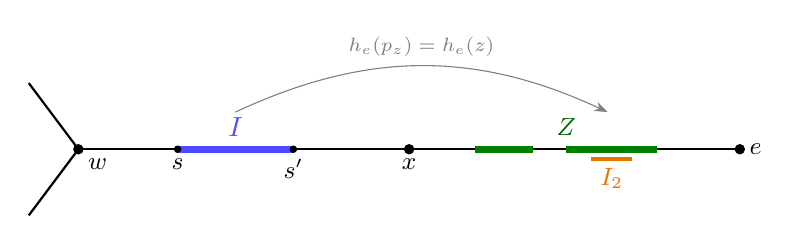
\begin{tikzpicture}[scale=1.05]
\draw[thick] (0,0)--(8,0);
\draw[thick] (0,0)--(-0.6,0.8); \draw[thick] (0,0)--(-0.6,-0.8);
\fill (0,0) circle (1.8pt) node[below right]{\small $w$};
\draw[line width=2.4pt,blue!70] (1.2,0)--(2.6,0) node[midway,above]{$I$};
\fill (1.2,0) circle (1.3pt) node[below]{\small $s$};
\fill (2.6,0) circle (1.3pt) node[below]{\small $s'$};
\fill (4.0,0) circle (1.8pt) node[below]{\small $x$};
\draw[line width=2.4pt,green!50!black] (4.8,0)--(5.5,0);
\draw[line width=2.4pt,green!50!black] (5.9,0)--(7.0,0);
\node[green!40!black,above] at (5.9,0.05) {\small $Z$};
\draw[line width=1.2pt,orange!90!black] (6.2,-0.12)--(6.7,-0.12);
\node[orange!90!black,below] at (6.45,-0.12) {\small $I_2$};
\fill (8,0) circle (1.8pt) node[right]{\small $e$};
\draw[->,>=Stealth,gray] (1.9,0.45) to[bend left=25] node[above,font=\scriptsize]{$h_{e}(p_z)=h_{e}(z)$} (6.4,0.45);
\end{tikzpicture}
\caption{Lemma~\ref{lem:matching} and Case~2 of Lemma~\ref{lem:ownedge} (schematic). The matching set $Z$ is open but possibly disconnected, and it lies on the sphere beyond $x$. In Lemma~\ref{lem:ownedge}, where the other end $w$ of the edge is a branch point, a closed subarc $I_2\subset Z$ is a spherical arc with the center $x$ between $w$ and $I_2$.}\label{fig:ownedge}
\end{figure}

\begin{lemma}[No center in the arc's own edge]\label{lem:ownedge}
Let $T$ be branched. If a spherical arc $I$ with center $x$ lies in the open edge $\ell^\circ$ of an edge $\ell$, then $x\notin\ell^\circ$.
\end{lemma}

\begin{role}
Together with Lemma~\ref{lem:tips}, this shows that the center of a spherical arc lies away from the arc's own edge and away from the tips. The boundary argument of Lemma~\ref{lem:boundary} reduces to exactly these two cases.
\end{role}

\begin{proof}
Suppose $x\in\ell^\circ$, and shrink $I$ to a closed arc in $\ell^\circ$. Let $K$ be the component of $S(x,r)$ containing $I$. By Lemma~\ref{lem:crossing} applied to $K$, for distinct $p,q\in I$ we have $\M(p,q)=\{x,y\}$ with $y\in(p,q)$, and $x$ is a crossing. Since $T$ is branched, $\ell$ has an end $w$ that is a branch point (see the paragraph after Lemma~\ref{lem:treestructure}). Orient $\ell$ away from $w$.

\emph{Case 1: $x$ lies between $w$ and $I$.} Take $p<q$ in $I$. On $(x,p]$ there is no zero and $f_{p,q}(p)<0$. Since $x$ is a crossing, $f_{p,q}>0$ just beyond $x$ towards $w$; with no further zero, $f_{p,q}(w)>0$. That is, $h_w(p)>h_w(q)$. But $[w,q]$ is an arc from the branch point $w$ passing through $p$ before $q$, so Lemma~\ref{lem:radial} gives $h_w(p)\le h_w(q)$. This is a contradiction.

\emph{Case 2: $I$ lies between $w$ and $x$.} If the other end of $\ell$ is a branch point, reverse the orientation and use Case~1. So let the other end be a tip $e$; see Figure~\ref{fig:ownedge}. Write $I=[s,s']$ with $s<s'<x<e$. By Lemma~\ref{lem:matching}, the set $Z$ defined there is a nonempty open subset of $S(x,r)\cap(x,e)$. Choose a closed nondegenerate arc $I_2\subset Z$. It is a spherical arc in $\ell^\circ$ with center $x$, and $x$ lies between $w$ and $I_2$. Case~1 applied to $I_2$ gives a contradiction.
\end{proof}

% =====================================================================
\section{Distances to the tips}\label{sec:tips}

In this section $T$ has a branch point. The next lemma is the analytic heart of the paper. It shows that certain ties at a tip cannot be ``flipped'' by moving a site; see Figure~\ref{fig:boundary}.

\begin{lemma}[No flip at a tip]\label{lem:boundary}
Let $T$ be branched, and let $e$ be a tip, and let $a,b$ be distinct edge points that lie either in one open edge, or in two open edges with a common end $v$. Suppose that $h_e(a)=h_e(b)$ and $f_{a,b}(u)\ne0$ for every vertex $u\ne e$. Then $a$ is a local extremum of $h_e$ on its open edge.
\end{lemma}

\begin{role}
This lemma gives strict monotonicity of tip distances (Proposition~\ref{prop:tipdistance}), which drives the counting in Sections~\ref{sec:count}--\ref{sec:triod}. Its proof follows an odd family of pairs to its boundary. There, the common center provided by Proposition~\ref{prop:oddbox} must become a midset point, and Lemmas~\ref{lem:tips} and \ref{lem:ownedge} exclude both candidates.
\end{role}

\begin{proof}
Let $\ell_a^\circ,\ell_b^\circ$ be the open edges containing $a,b$ (they coincide if $a,b$ share an open edge). Since the only possible vertex on $[a,b]$ is $v$, which is not a zero, we have $\M(a,b)=\{e,y\}$ with $y$ an edge point in $\ell_a^\circ\cup \ell_b^\circ$. Suppose $a$ is not a local extremum of $h_e$ on $\ell_a^\circ$; we derive a contradiction in five steps: freeze the signs (Step~1), find an odd segment ending at a tie (Step~2), fix one center along it (Step~3), carry that center to the tie (Step~4), and exclude it (Step~5).

\emph{Step 1: a box with frozen signs.} Choose disjoint open arcs $U\ni a$ in $\ell_a^\circ$ and $V\ni b$ in $\ell_b^\circ$ so small that, for all $(a',b')\in U\times V$ and all vertices $u\ne e$, the sign of $f_{a',b'}(u)$ is nonzero and equals that of $f_{a,b}(u)$. In particular the number
\[
  N_0=\bigl|\{u\in\Odd\setminus\{e\}:\ f_{a',b'}(u)<0\}\bigr|
\]
is the same for all $(a',b')\in U\times V$. If $f_{a',b'}(e)\ne0$, the pair $(a',b')$ is strict and $\N(a',b')=N_0+[f_{a',b'}(e)<0]$, since $e\in\Odd$. Put $\eta=-1$ if $N_0$ is even and $\eta=+1$ if $N_0$ is odd. Then every $(a',b')\in U\times V$ with $\sgn f_{a',b'}(e)=\eta$ is strict with $\N(a',b')$ odd.

\emph{Step 2: an odd segment ending at a tie.} Since $a$ is not a local extremum of $h_e$, there is $s_1\in U$ with $\sgn f_{s_1,b}(e)=\eta$. Let $a_0$ be the point of the closed arc $[a,s_1]$ nearest to $s_1$ with $h_e(a_0)=h_e(b)$; it exists because this set is closed and contains $a$. On $L=(a_0,s_1]$ the function $f_{\cdot,b}(e)$ has no zero, so it has sign $\eta$ throughout. Ties at $e$ may accumulate at $a$, but $L$ always ends at a tie.

\emph{Step 3: one center along $L$ (equality, not a limit).} For each $s\in L$ the pair $(s,b)$ is strict with $\N(s,b)$ odd. Corollary~\ref{cor:oddpair} gives a center $c_s$, a radius $r_s>0$, and open arcs $P_s\ni s$ in $\ell_a^\circ$ and $Q_s\ni b$ in $\ell_b^\circ$ with $P_s\cup Q_s\subset S(c_s,r_s)$. (These arcs come from Corollary~\ref{cor:oddpair}; they are unrelated to the arcs $U,V$ of Step~1.) Let $s,s'\in L$. Both $Q_s$ and $Q_{s'}$ are open arcs in $\ell_b^\circ$ containing $b$, so $Q_s\cap Q_{s'}$ is a nondegenerate arc. It is spherical with center $c_s$ and with center $c_{s'}$. By the uniqueness of centers (Lemma~\ref{lem:sphericalarc}(b)), $c_s=c_{s'}$. This is an equality for every pair $s,s'\in L$; no limit of centers is taken. Writing $c$ for the common center, we have the invariant
\begin{equation}\label{eq:invariant}
  c_s=c,\qquad r_s=d(c,b)=:r,\qquad d(c,s)=d(c,b)=r\qquad(s\in L).
\end{equation}

\emph{Step 4: passage to the boundary.} The tie $a_0$ is an end of $L$, and $h_c$ is continuous. By \eqref{eq:invariant}, $d(c,a_0)=r=d(c,b)$, that is,
\begin{equation}\label{eq:boundary}
  c\in\M(a_0,b).
\end{equation}

\emph{Step 5: the boundary midset and the exclusion.} Since $a_0\in[a,s_1]\subset U$, Step~1 shows that every vertex $u\ne e$ has $f_{a_0,b}(u)\ne0$, while $f_{a_0,b}(e)=0$. Also $a_0\ne b$, because $U\cap V=\emptyset$. By the DMP and the intermediate value principle on $[a_0,b]$, the second zero $y_0$ is a point of $(a_0,b)$ that is not a vertex. The open arc $(a_0,b)$ lies in $\ell_a^\circ$ if $a,b$ share an open edge, and in $\ell_a^\circ\cup\{v\}\cup\ell_b^\circ$ otherwise. Together with \eqref{eq:boundary} this gives
\[
  c\in\M(a_0,b)=\{e,y_0\},\qquad y_0\in\ell_a^\circ\cup\ell_b^\circ .
\]
By Corollary~\ref{cor:oddpair}, $c$ is an edge point, so $c\ne e$. (Alternatively, $c=e$ would contradict Lemma~\ref{lem:tips}.) Hence $c=y_0$. If $y_0\in\ell_a^\circ$, then $c$ is the center of a spherical arc in its own open edge, namely a closed subarc of $P_s$. If $y_0\in\ell_b^\circ$, the same holds with $Q_s$. Either way this contradicts Lemma~\ref{lem:ownedge}.
\end{proof}

\begin{figure}[ht]
\centering
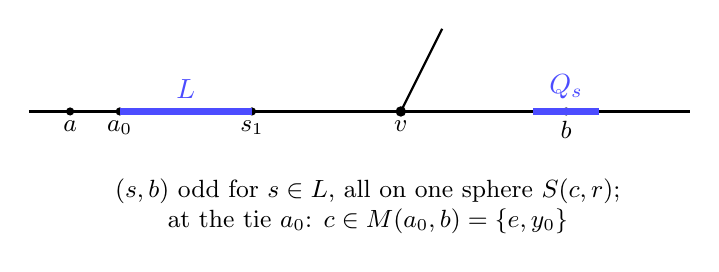
\begin{tikzpicture}[scale=1.05]
\draw[thick] (-4.5,0)--(0,0)--(3.5,0);
\draw[thick] (0,0)--(0.5,1.0);
\fill (0,0) circle (1.8pt) node[below]{\small $v$};
\fill (-4.0,0) circle (1.4pt) node[below]{\small $a$};
\fill (-3.4,0) circle (1.4pt) node[below]{\small $a_0$};
\fill (-1.8,0) circle (1.4pt) node[below]{\small $s_1$};
\draw[line width=2.4pt,blue!70] (-3.4,0)--(-1.8,0) node[midway,above]{$L$};
\fill (2.0,0) circle (1.4pt) node[below]{\small $b$};
\draw[line width=2.4pt,blue!70] (1.6,0)--(2.4,0) node[midway,above]{$Q_s$};
\node[font=\small,align=center] at (-0.4,-1.15) {$(s,b)$ odd for $s\in L$, all on one sphere $S(c,r)$;\\ at the tie $a_0$: $c\in\M(a_0,b)=\{e,y_0\}$};
\end{tikzpicture}
\caption{Lemma~\ref{lem:boundary}. The odd segment $L$ ends at a tie $a_0$, where the common center $c$ becomes a midset point. Neither candidate for $c$ is possible. Schematic: positions carry no metric meaning.}\label{fig:boundary}
\end{figure}

\begin{proposition}[Distances to tips]\label{prop:tipdistance}
Let $e$ be a tip of the branched tree $T$.
\begin{enumerate}[label=\textup{(\alph*)}]
\item $h_e$ is strictly monotone on every edge.
\item If $v$ is a branch point and $a,b$ lie in two distinct open edges at $v$ with $h_e(a)=h_e(b)$, then $h_v(a)=h_v(b)$.
\end{enumerate}
\end{proposition}

\begin{role}
Part (a) lets us speak of each tip's distance increasing or decreasing along each edge; this is the data that is counted in Sections~\ref{sec:count} and \ref{sec:triod}. Part (b) says that ties seen by a tip through a branch point are also seen by the branch point.
\end{role}

\begin{proof}
(a) Let $p\ne q$ be in one open edge $\ell'^\circ$ with $h_e(p)=h_e(q)$. By Lemma~\ref{lem:tips}, $h_e$ is not constant on $[p,q]$; say it exceeds $h_e(p)$ somewhere on $(p,q)$ (the other case is symmetric). Let $\mu$ be its maximum on $[p,q]$. By Lemma~\ref{lem:extrema}(i), choose $\lambda\in(h_e(p),\mu)$ that is not a local extremum value of $h_e$ on $\ell'^\circ$, and choose $a,b\in(p,q)$ on either side of a maximum point with $h_e(a)=h_e(b)=\lambda$. Then $\M(a,b)=\{e,y\}$ with $y\in(a,b)\subset \ell'^\circ$, so $f_{a,b}(u)\ne0$ for every vertex $u\ne e$. By Lemma~\ref{lem:boundary}, $a$ is a local extremum of $h_e$, which contradicts the choice of $\lambda$. So $h_e$ is injective on each open edge, hence strictly monotone there and, by continuity, on each edge.

(b) If $h_v(a)\ne h_v(b)$, then $\M(a,b)=\{e,y\}$ with $y\in(a,b)\setminus\{v\}$, so $f_{a,b}(u)\ne0$ for every vertex $u\ne e$. By Lemma~\ref{lem:boundary}, $a$ is a local extremum of $h_e$ on its edge, contradicting (a).
\end{proof}

% =====================================================================
\section{Counting tips}\label{sec:count}

\begin{definition}[Directions and used pairs]\label{def:uses}
Let $v$ be a branch point of the branched tree $T$ and $e$ a tip. By Proposition~\ref{prop:tipdistance}(a), on each edge at $v$ the function $h_e$ is either strictly increasing or strictly decreasing in the direction away from $v$. We say that $e$ \emph{uses} the unordered pair $\{\ell,\ell'\}$ of distinct edges at $v$ if $h_e$ has the same direction on $\ell$ and on $\ell'$.
\end{definition}

\begin{lemma}[Distinct tips use disjoint pairs]\label{lem:pairs}
Let $T$ be branched. At a branch point $v$ of $T$, no pair of edges is used by two distinct tips.
\end{lemma}

\begin{proof}
Let $\ell,\ell'$ be edges at $v$, and suppose the tips $e\ne e'$ both use $\{\ell,\ell'\}$. By Lemma~\ref{lem:radial}, $h_v$ is nondecreasing along $\ell$ and $\ell'$ away from $v$, with $h_v(v)=0$. Let $u,u'$ be the far ends of $\ell,\ell'$ and $R=\min\{h_v(u),h_v(u')\}>0$. For $\rho\in(0,R)$ the level set $\{h_v=\rho\}\cap\ell$ is nonempty by the intermediate value theorem. It is a point or a nondegenerate arc, since $h_v$ is monotone on $\ell$, and it lies in $\ell^\circ$, since $h_v(v)=0<\rho<h_v(u)$. The nondegenerate levels on $\ell$ are disjoint arcs, so only countably many values $\rho$ give them; the same holds on $\ell'$. Choose $\rho_k\in(0,R)$, $\rho_k\to0$, avoiding both countable sets. The \emph{radial matching} then pairs the unique points $a_k\in\ell^\circ$ and $b_k\in\ell'^\circ$ with $h_v(a_k)=h_v(b_k)=\rho_k$. Any limit point of $(a_k)$ is at distance $0$ from $v$, so $a_k\to v$; likewise $b_k\to v$.

Since $e$ uses the pair, $h_e$ moves away from $h_e(v)$ in the same direction on both edges, strictly by Proposition~\ref{prop:tipdistance}(a). So for $a\in\ell^\circ$ close enough to $v$, the value $h_e(a)$ lies strictly between $h_e(v)$ and $h_e(u')$, and there is a unique $b=\mu_e(a)\in\ell'^\circ$ with $h_e(b)=h_e(a)$. We call $\mu_e$ the \emph{$e$-matching}; it should not be confused with the radial matching. By Proposition~\ref{prop:tipdistance}(b), $h_v(\mu_e(a))=h_v(a)$: the $e$-matching preserves the radial level. Taking $a=a_k$ with $k$ large, this forces $\mu_e(a_k)=b_k$, because $h_v(b)=\rho_k$ and the $\rho_k$-level of $h_v$ on $\ell'$ is $\{b_k\}$; so $h_e(a_k)=h_e(b_k)$. The same holds for $e'$. Then $\M(a_k,b_k)\supset\{v,e,e'\}$, a contradiction.
\end{proof}

\begin{proposition}[Reduction to the triod]\label{prop:triod}
A branched finite tree with the DMP is a simple triod.
\end{proposition}
\begin{proof}
Let $v$ be a branch point. By Lemma~\ref{lem:order} its degree $m$ is $3$ or $4$. If $k$ of the edges at $v$ are increasing for a tip $e$, then $e$ uses $\binom k2+\binom{m-k}2$ pairs. This is at least $1$ when $m=3$ and at least $2$ when $m=4$. There are $\binom m2$ pairs, used by distinct tips disjointly (Lemma~\ref{lem:pairs}), so $T$ has at most $3$ tips in both cases. By \eqref{eq:tips} the number of tips is at least $m$, so $m=3$, and every branch point has degree $3$. Then \eqref{eq:tips} gives $t=2+|B|\le3$, so $T$ has exactly one branch point and three tips, that is, $T$ is a simple triod.
\end{proof}

% =====================================================================
\section{The simple triod}\label{sec:triod}

\begin{theorem}\label{thm:triod}
No compatible metric on a simple triod has the DMP.
\end{theorem}

\begin{proof}
Let $T$ be a simple triod with center $v$, tips $e_1,e_2,e_3$ and legs $\ell_j=[v,e_j]$, and suppose $d$ has the DMP. Put $r_i=d(v,e_i)$. By Proposition~\ref{prop:tipdistance}(a), each $h_{e_i}$ is strictly monotone on each leg. Record in a $3\times3$ table the direction of $h_{e_i}$ along $\ell_j$, moving away from $v$: entry $(i,j)$ is $\downarrow$ (decreasing) or $\uparrow$ (increasing). Each diagonal entry is $\downarrow$, since $h_{e_j}(e_j)=0$.

\emph{(i) No row has three $\downarrow$.} A tip with three decreasing legs would use all three pairs of legs. By Lemma~\ref{lem:pairs} no pair would then be left for the other two tips, which each use at least one pair.

\emph{(ii) Every column has exactly two $\downarrow$.} Fix $j$. Since $h_v$ is nondecreasing along $\ell_j$ (Lemma~\ref{lem:radial}) and is positive at $e_j$, there are edge points $p,q\in\ell_j$, with $p$ before $q$, such that $h_v(p)<h_v(q)$. By Proposition~\ref{prop:tipdistance}(a), $f_{p,q}(e_i)\ne0$ for each tip $e_i$, and $f_{p,q}(v)\ne0$ by the choice of $p,q$; so $(p,q)$ is strict. By \eqref{eq:signconv}, the vertices counted by $\N(p,q)$ are those whose distance increases from $p$ to $q$. These are $v$, which is counted, and the tips $e_i$ with an $\uparrow$ in column $j$; the tip $e_j$ is not counted.

Suppose $\N(p,q)$ were odd. By Corollary~\ref{cor:oddpair} there are a center $c$ and an open arc $P\ni p$ in $\ell_j$ with $P\subset S(c,\rho)$ for some $\rho>0$. By Corollary~\ref{cor:oddpair}, $c$ is an edge point (in particular $c\ne v$, as also follows from $h_v(p)\ne h_v(q)$). Take $p'$ before $q'$ in $P$. By Lemma~\ref{lem:crossing}, $\N(p',q')$ is even. But the tip signs of $(p',q')$ equal those of $(p,q)$, by the strict monotonicity of tip distances on $\ell_j$ (Proposition~\ref{prop:tipdistance}(a)). The sign at $v$ also agrees: $h_v$ is nondecreasing on $\ell_j$ and strictly monotone on a closed subarc of $P$ containing $p',q'$ (Lemma~\ref{lem:sphericalarc}(a), as $v\notin P$ and $v\ne c$), hence increasing there. So $\N(p',q')=\N(p,q)$, a contradiction.

Thus $\N(p,q)$ is even. Since $v$ is counted and $e_j$ is not, exactly one of the other two tips has an $\uparrow$ in column $j$, and column $j$ has exactly two $\downarrow$.

\emph{(iii) The cycle.} By (ii) the table has six $\downarrow$. By (i) each row has at most two, so each row has exactly two: the diagonal one and one more. Hence every row and every column has exactly one off-diagonal $\downarrow$. Write $i\to j$ if entry $(i,j)$, $i\ne j$, is $\downarrow$. This defines a permutation of $\{1,2,3\}$ without fixed points, that is, a cyclic permutation; see Figure~\ref{fig:triod}.

If $i\to j$, then $h_{e_i}$ decreases along $\ell_j$, so $r_i=h_{e_i}(v)>h_{e_i}(e_j)=d(e_i,e_j)$. In a $3$-cycle $j\not\to i$, so $h_{e_j}$ increases along $\ell_i$, giving $r_j=h_{e_j}(v)<h_{e_j}(e_i)=d(e_i,e_j)$. Hence $i\to j$ implies $r_i>r_j$. Going once around the cycle yields $r_1>r_1$, which is absurd.
\end{proof}

\begin{figure}[ht]
\centering
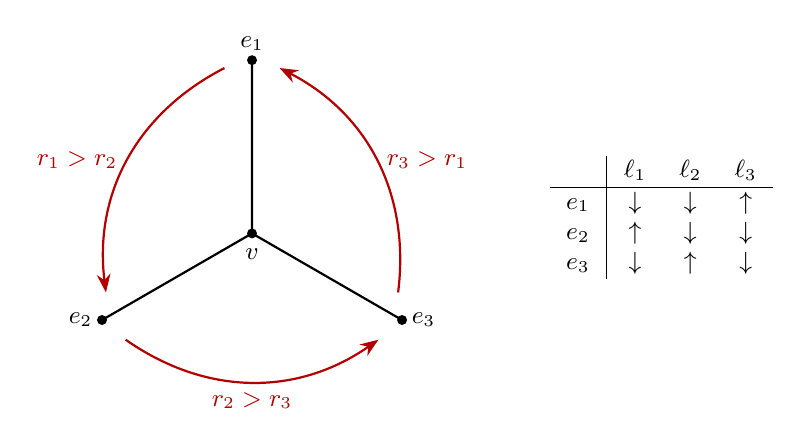
\begin{tikzpicture}[scale=1.0,>=Stealth]
\coordinate (v) at (0,0);
\coordinate (e1) at (90:2.2); \coordinate (e2) at (210:2.2); \coordinate (e3) at (330:2.2);
\draw[thick] (v)--(e1) (v)--(e2) (v)--(e3);
\fill (v) circle (1.8pt) node[below=2pt]{\small $v$};
\foreach \p/\n/\pos in {e1/e_1/above,e2/e_2/left,e3/e_3/right} \fill (\p) circle (1.8pt) node[\pos]{\small $\n$};
\draw[->,red!70!black,thick] ($(e1)+(-0.35,-0.1)$) to[bend right=35] node[left,font=\small]{$r_1>r_2$} ($(e2)+(0.05,0.35)$);
\draw[->,red!70!black,thick] ($(e2)+(0.3,-0.25)$) to[bend right=35] node[below,font=\small]{$r_2>r_3$} ($(e3)+(-0.3,-0.25)$);
\draw[->,red!70!black,thick] ($(e3)+(-0.05,0.35)$) to[bend right=35] node[right,font=\small]{$r_3>r_1$} ($(e1)+(0.35,-0.1)$);
\node[font=\small,align=left] at (5.2,0.2) {
\begin{tabular}{c|ccc}
 & $\ell_1$ & $\ell_2$ & $\ell_3$\\ \hline
$e_1$ & $\downarrow$ & $\downarrow$ & $\uparrow$\\
$e_2$ & $\uparrow$ & $\downarrow$ & $\downarrow$\\
$e_3$ & $\downarrow$ & $\uparrow$ & $\downarrow$
\end{tabular}};
\end{tikzpicture}
\caption{The forced pattern in Theorem~\ref{thm:triod}, shown for the cycle $1\to2\to3\to1$. Each arrow $i\to j$ gives $r_i>d(e_i,e_j)>r_j$, and the cycle is impossible. The drawing is topological; the leg lengths $r_i$ are metric quantities not represented by the picture.}\label{fig:triod}
\end{figure}

% =====================================================================
\section{The arc}\label{sec:arc}

\begin{theorem}\label{thm:arc}
No compatible metric on an arc has the DMP.
\end{theorem}

\begin{proof}
Let $T=[0,1]$, with the usual order, carry a compatible metric with the DMP. The vertices are $0$ and $1$, both of odd degree. Sections~\ref{sec:signs}--\ref{sec:spheres} and Lemmas~\ref{lem:tips}, \ref{lem:crossing} and \ref{lem:matching} apply, since none of them requires a branch point.

\emph{A sphere.} For $a$ near $0$ and $b$ near $1$ we have $f_{a,b}(0)<0<f_{a,b}(1)$, so $(a,b)$ is strict with $\N(a,b)=1$. By Corollary~\ref{cor:oddpair}, $a$ and $b$ are interior points of spherical arcs with a common center $x$ and radius $r$. By Corollary~\ref{cor:oddpair}, $x$ is an edge point, so $0<x<1$. Put $\Sigma=S(x,r)$; it is closed and $x\notin\Sigma$.

Throughout, the center $x$ and the radius $r$ are fixed, and every point produced below lies on this same sphere $\Sigma$. The arc $[0,1]$ is a single edge whose two ends are tips. So Lemma~\ref{lem:matching} applies in both directions: towards the tip $e=1$ for spherical arcs in $(0,x)$, and towards the tip $e=0$ for spherical arcs in $(x,1)$.

\emph{Step 1 (matching to the right).} Let $a$ be an interior point of a nondegenerate arc in $\Sigma\cap(0,x)$. Then there is $b\in\Sigma\cap(x,1)$, interior to a nondegenerate arc in $\Sigma\cap(x,1)$, with $h_1(b)=h_1(a)$ and $h_0(a)<h_0(b)$.

Indeed, choose $s<a<s'$ with $I=[s,s']\subset\Sigma\cap(0,x)$. The points $s,s',x,1$ occur in this order, so Lemma~\ref{lem:matching} with $e=1$ applies. By part~(b) the open set $Z$ contains a point $b$ with $h_1(b)=h_1(a)$, and by part~(c), $Z$ is an open subset of $\Sigma\cap(x,1)$; so $b$ is interior to a nondegenerate arc in $\Sigma\cap(x,1)$. Also by part~(c), applied with $p_b=a$, we have $\M(a,b)=\{1,x\}$. Both zeros lie beyond $a$, so $f_{a,b}$ has no zero on $[0,a]$, and $f_{a,b}(0)$ has the sign of $f_{a,b}(a)<0$. That is, $h_0(a)<h_0(b)$.

\emph{Step 2 (matching to the left).} Let $b$ be an interior point of a nondegenerate arc in $\Sigma\cap(x,1)$. Then there is $a'\in\Sigma\cap(0,x)$, interior to a nondegenerate arc in $\Sigma\cap(0,x)$, with $h_0(a')=h_0(b)$.

Indeed, choose a closed arc $I\subset\Sigma\cap(x,1)$ having $b$ in its interior, and call its ends $s$ (the one nearer $1$) and $s'$ (the one nearer $x$). Then $s,s',x,0$ occur in this order along the edge towards the tip $0$, so Lemma~\ref{lem:matching} with $e=0$ applies. It gives a point $a'$ with $h_0(a')=h_0(b)$ in an open subset of $\Sigma\cap(0,x)$.

\emph{Iteration.} One of the sites $a<b$ of the first paragraph ($a$ near $0$, $b$ near $1$) lies on the correct side of $x$: since $a\ne x\ne b$, either $a<x$, or $x<a<b$. In the first case put $a_1=a$. In the second case $b$ is an interior point of a spherical arc in $\Sigma\cap(x,1)$, and Step~2 provides $a_1$. Starting from $a_1$ and alternating Steps~1 and 2 produces points $a_1,b_1,a_2,b_2,\dots$ of $\Sigma$ with $a_n<x<b_n$. Each $a_n$ is interior to a nondegenerate arc in $\Sigma\cap(0,x)$, and each $b_n$ to one in $\Sigma\cap(x,1)$, so both steps can be repeated indefinitely. What increases is not the position of these points but the numbers
\[
  A_n=h_0(a_n),\qquad B_n=h_0(b_n),\qquad\text{which satisfy}\qquad A_n<B_n=A_{n+1},
\]
together with $h_1(a_n)=h_1(b_n)$ for all $n$ (Figure~\ref{fig:arc}).

\emph{Limit.} The sequence $(A_n)$ is increasing and bounded by $\diam T$, hence convergent. So $B_n-A_n=A_{n+1}-A_n\to0$. By compactness pass to a subsequence with $a_n\to a_*$ and $b_n\to b_*$. Since $a_n\in\Sigma\cap[0,x)$, $b_n\in\Sigma\cap(x,1]$, $\Sigma$ is closed and $x\notin\Sigma$, we get $a_*\in\Sigma\cap[0,x)$ and $b_*\in\Sigma\cap(x,1]$. In particular $a_*<x<b_*$, so the limiting sites are distinct. By continuity, $h_1(a_*)=h_1(b_*)$ and $h_0(a_*)=h_0(b_*)$, while $h_x(a_*)=r=h_x(b_*)$. Note that $a_*\ne0$: otherwise $h_0(b_*)=h_0(a_*)=0$ would force $b_*=0=a_*$. Likewise $b_*\ne1$. So $0$, $x$ and $1$ are three distinct points of $\M(a_*,b_*)$, a contradiction.
\end{proof}

\begin{figure}[ht]
\centering
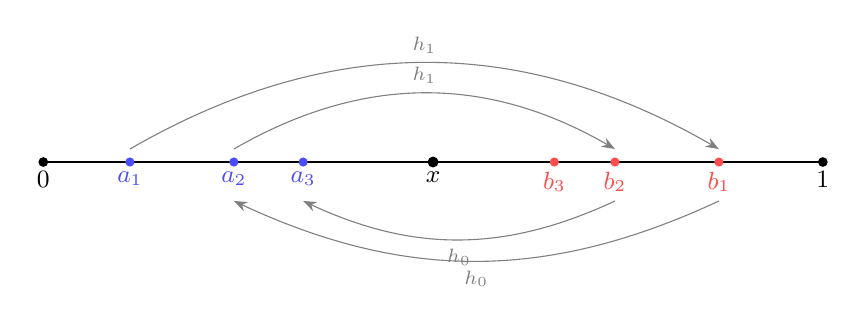
\begin{tikzpicture}[scale=1.1,>=Stealth]
\draw[thick] (0,0)--(9,0);
\fill (0,0) circle (1.6pt) node[below]{\small $0$};
\fill (9,0) circle (1.6pt) node[below]{\small $1$};
\fill (4.5,0) circle (1.8pt) node[below]{\small $x$};
\foreach \a/\l in {1.0/1,2.2/2,3.0/3} {\fill[blue!70] (\a,0) circle (1.5pt); \node[below,blue!70] at (\a,0) {\small $a_\l$};}
\foreach \b/\l in {7.8/1,6.6/2,5.9/3} {\fill[red!70] (\b,0) circle (1.5pt); \node[below,red!70] at (\b,0) {\small $b_\l$};}
\draw[->,gray] (1.0,0.15) to[bend left=30] node[above,font=\scriptsize]{$h_1$} (7.8,0.15);
\draw[->,gray] (7.8,-0.45) to[bend left=25] node[below,font=\scriptsize]{$h_0$} (2.2,-0.45);
\draw[->,gray] (2.2,0.15) to[bend left=30] node[above,font=\scriptsize]{$h_1$} (6.6,0.15);
\draw[->,gray] (6.6,-0.45) to[bend left=25] node[below,font=\scriptsize]{$h_0$} (3.0,-0.45);
\end{tikzpicture}
\caption{Theorem~\ref{thm:arc}, schematic. Distances to $1$ match $a_n$ with $b_n$, and distances to $0$ match $b_n$ with $a_{n+1}$. The positions drawn are illustrative only: the proof controls the increasing values $A_n=h_0(a_n)$, not the order of the points along the arc. In the limit the pair $(a_*,b_*)$ is equidistant from $0$, $x$ and $1$.}\label{fig:arc}
\end{figure}

% =====================================================================
\section{Proofs of the main theorems}\label{sec:proofs}

\begin{proof}[Proof of Theorem~\ref{thm:B}]
Let $T$ be a finite tree with a compatible DMP metric. If $T$ has a branch point, it is a simple triod by Proposition~\ref{prop:triod}, which is impossible by Theorem~\ref{thm:triod}. Otherwise $T$ is an arc, which is impossible by Theorem~\ref{thm:arc}.
\end{proof}

\begin{proof}[Proof of Theorem~\ref{thm:C}]
This is Lemma~\ref{lem:order}, Theorem~\ref{thm:branchcount} and Corollary~\ref{cor:finitetree}.
\end{proof}

\begin{proof}[Proof of Theorem~\ref{thm:A}]
Let $(X,d)$ be a continuum with the DMP. By Corollary~\ref{cor:dendrite}, $X$ is a simple closed curve or a dendrite. If $X$ were a dendrite, it would be a finite tree by Corollary~\ref{cor:finitetree}, which Theorem~\ref{thm:B} excludes. Hence $X$ is a simple closed curve.

Conversely, the unit circle in $\mathbb R^2$ with the Euclidean metric has the DMP. For distinct $a,b$ on it, $\M(a,b)$ is the intersection of the circle with the perpendicular bisector of $ab$, a line through the center, which consists of two points.
\end{proof}

% =====================================================================
\section{Remarks and questions}\label{sec:remarks}

\subsection{Where the hypotheses are used}
The argument uses the cardinality hypothesis at three strengths.
\begin{itemize}[leftmargin=*]
\item Finiteness of midsets suffices for local connectedness (Proposition~\ref{prop:lc}).
\item The upper bound $|\M(a,b)|\le2$ suffices for the circle case (Proposition~\ref{prop:circle}), for all of Section~\ref{sec:branch}, and for the uniqueness and monotonicity properties of spherical arcs (Lemma~\ref{lem:sphericalarc}).
\item The exact value two is used from Corollary~\ref{cor:types} on. It guarantees that each strict pair has a second zero, which is a touch when $\N$ is odd, and that the two midset points stay apart on a Baire-large set of pairs (Lemma~\ref{lem:selection}).
\end{itemize}
The upper bound alone does not exclude branching. Two straight segments in the Euclidean plane, crossing at their midpoints at an angle different from $\pi/2$, form a four-armed star in which every midset has at most two points. Indeed, a perpendicular bisector meets each segment in at most one point unless it contains that segment. It contains a segment only if the two sites are mirror images in that segment's line. A reflection in one of the lines maps the other line to itself only when the lines are perpendicular. Hence a site on the other segment, other than the common point, has its mirror image off the star, while a site on the line of reflection is its own image; in neither case are there two distinct sites. This star is a dendrite as in Theorem~\ref{thm:C} with one branch point of order four, so Lemma~\ref{lem:order} is sharp. We do not know whether the bound $|B|\le4$ of Theorem~\ref{thm:C} is attained.

\subsection{Questions}
Spaces in which every midset is a single point (the unique midset property) were studied by Berard \cite{Ber71} and Nadler \cite{Nad76}; the Euclidean arc is an example. Loveland showed that no arc or simple closed curve in the plane has the triple midset property \cite{Lov90}. For plane continua with the Euclidean metric, Loveland and Loveland deduced from \cite[Theorem~3.1]{LL92} that a continuum in which all midsets are finite with the same cardinality is an arc or a simple closed curve; see the introduction of \cite{LL92}. Our methods suggest the following problem for arbitrary metrics.

\begin{question}
Let $(X,d)$ be a continuum and $n\ge1$ an integer such that $|\M(a,b)|=n$ for all distinct $a,b\in X$. Must $n\le2$? Must $X$ then be an arc ($n=1$) or a simple closed curve ($n=2$)?
\end{question}

\noindent
Proposition~\ref{prop:lc} shows that such an $X$ is locally connected, and the parity count of Lemma~\ref{lem:parity} is available on any finite tree. Theorem~\ref{thm:B} settles the case $n=2$ for finite trees; a natural first step would be to decide whether the methods of Sections~\ref{sec:signs}--\ref{sec:arc} give $n\le2$ for finite trees. Loveland also studied Apollonius sets $\{x:d(x,a)=\lambda d(x,b)\}$ for a fixed ratio $\lambda>0$ \cite{L76b}. It would be interesting to know whether the arguments of Sections~\ref{sec:signs}--\ref{sec:arc} extend to $\lambda\ne1$.

\subsection{Higher dimensions}
For $n\ge0$, a metric space has the \emph{$n$-sphere midset property} if every midset $\M(a,b)$ with $a\ne b$ is homeomorphic to the $n$-sphere $S^n$. Since $S^0$ is a two-point space, the $0$-sphere midset property is the DMP. On the round sphere $S^n\subset\mathbb R^{n+1}$ with the Euclidean metric, the midset of two distinct points is the intersection of $S^n$ with their perpendicular bisector, a hyperplane through the center, so it is a great $(n-1)$-sphere. Thus $S^n$ has the $(n-1)$-sphere midset property. Hattori \cite{H01} records the following conjecture, which would characterize $S^n$ in the way Theorem~\ref{thm:A} characterizes $S^1$.

\begin{conjecture}[The $(n-1)$-sphere midset conjecture]\label{conj:sphere}
Let $n\ge1$ and let $(X,d)$ be a continuum with the $(n-1)$-sphere midset property. Then $X$ is homeomorphic to $S^n$.
\end{conjecture}

\noindent
Hattori states the conjecture for nondegenerate compact metric spaces. For $n=1$ connectedness cannot be dropped: four points at mutual distance $1$ form a compact metric space with the DMP, since the midset of any two of them consists of the other two. For continua, the case $n=1$ is Theorem~\ref{thm:A}. For $n=2$, Loveland proved that a metric space with the $1$-sphere midset property is a $2$-sphere if it contains a subset homeomorphic to $S^2$, and that a nondegenerate compact metric space with the $1$-sphere midset property is a $2$-sphere if every simple closed curve separates it \cite{Lov77}; see \cite[Theorem~8]{H01}. A theorem recorded in \cite{H01} says that a separable metrizable space admitting a totally bounded metric whose midsets all have dimension at most $n-1$ has dimension at most $n$. Since a compact metric is totally bounded, a continuum as in Conjecture~\ref{conj:sphere} has $\dim X\le n$.

\begin{question}\label{q:sphere}
Let $n\ge2$.
\begin{enumerate}[label=(\alph*),leftmargin=*]
\item Is Conjecture~\ref{conj:sphere} true for $n=2$? That is, is every continuum in which all midsets of distinct points are simple closed curves homeomorphic to $S^2$?
\item Is a continuum with the $(n-1)$-sphere midset property locally connected, and is its dimension exactly $n$?
\item Is a nondegenerate compact metric space with the $(n-1)$-sphere midset property necessarily connected?
\end{enumerate}
\end{question}

\noindent
Part~(b) asks for the analogue of the first step of our proof, where finiteness of midsets gives local connectedness (Proposition~\ref{prop:lc}). The later steps use that a dendrite has many cut points and that $d(\cdot,a)-d(\cdot,b)$ changes sign along arcs; for $n\ge2$ one would need a substitute for the parity count of Lemma~\ref{lem:parity} on the components of the complement of a midset.

% =====================================================================
\section*{Formalization in Lean 4}

The results of this paper have been formalized in Lean~4 with the library Mathlib. The development is available at \url{https://github.com/LucasAlves8Sp/Double-midset-conjecture-for-metric-continua}, in the folder \texttt{lean/}. It was compiled with Lean \texttt{v4.35.0-rc2} and the Mathlib release of the same tag.

\emph{What is formalized.} Every definition, lemma, proposition, corollary and theorem of Sections~\ref{sec:prelim}--\ref{sec:proofs}, and the facts of Section~\ref{sec:prelim} in the form in which they are used: 47 statements in all, collected in the file \texttt{Challenge.lean}. They include Theorems~\ref{thm:A}, \ref{thm:B} and~\ref{thm:C}, the converse that the Euclidean circle has the DMP, and the resulting characterization: a metrizable continuum admits a compatible metric with the DMP if and only if it is a simple closed curve. The classical facts that are not in Mathlib, such as the existence of arcs in Peano continua and boundary bumping, are proved in the development. Every formal proof is complete, uses no axiom beyond the three standard ones of Lean with classical logic (\texttt{propext}, \texttt{Classical.choice}, \texttt{Quot.sound}), and was accepted by the Lean kernel and by the independent proof checkers run through the tool Comparator. The repository records exactly which checks were run and under which conditions.

\emph{What is not formalized.} The examples, the figures, the remarks and the questions of Section~\ref{sec:remarks}. R.~L. Moore's theorem (Fact~\ref{fact:notriod}) is formalized only in the consequence used here, that a dendrite without branch points is an arc, and equation~\eqref{eq:swap} only as the parity statement $\N(a,b)\equiv\N(b,a)\pmod 2$. Several formal statements are slightly more general than the written ones; the file \texttt{formalization.yaml} lists every divergence. The correspondence between the formal statements and the statements of the paper has so far been checked only by AI systems.

% =====================================================================
\section*{Disclosure of the use of artificial intelligence}

Artificial intelligence was used extensively in this work: to obtain the results, to proofread and write the paper, and to test the results adversarially. The models used were Claude Opus~5.5 (Anthropic), ChatGPT Astra~6.2 and ChatGPT Sol~6.1 (OpenAI). Claude Opus~5.5 was the main model for the proof of the first part of the argument, and ChatGPT Astra~6.2 for the triod and dendrite cases.

The author guided the work throughout. He proposed the subgoals and directed the proofs. Many rounds of review were carried out, in which proof attempts, reports and candidate results were produced and checked. The Lean code of the formalization described in the previous section, both statements and proofs, was written by Claude Opus~5.5 at the author's request.\par The author takes full responsibility for the content of this paper.

% =====================================================================
\begin{thebibliography}{99}

\bibitem{Ber71}
A.~D. Berard, Jr., \emph{Characterizations of metric spaces by the use of their midsets: intervals}, Fund. Math. \textbf{73} (1971/72), no.~1, 1--7. \href{https://doi.org/10.4064/fm-73-1-1-7}{doi:10.4064/fm-73-1-1-7}.

\bibitem{BN74}
A.~D. Berard, Jr. and W. Nitka, \emph{A new definition of the circle by the use of bisectors}, Fund. Math. \textbf{85} (1974), 49--55. \href{https://doi.org/10.4064/fm-85-1-49-55}{doi:10.4064/fm-85-1-49-55}.

\bibitem{CC00}
M.~N. Charatonik and W.~J. Charatonik, \emph{On Mazurkiewicz sets}, Comment. Math. Univ. Carolin. \textbf{41} (2000), no.~4, 817--819.

\bibitem{H01}
Y. Hattori, \emph{Special metrics}, in: Proceedings of the Ninth Prague Topological Symposium (Prague, 2001), Topology Atlas, Toronto, 2002, 155--164. \href{https://arxiv.org/abs/math/0204130}{arXiv:math/0204130}.

\bibitem{L76}
L.~D. Loveland, \emph{A metric characterization of a simple closed curve}, General Topology Appl. \textbf{6} (1976), 309--313. \href{https://doi.org/10.1016/0016-660X(76)90020-9}{doi:10.1016/0016-660X(76)90020-9}.

\bibitem{L76b}
L.~D. Loveland, \emph{Continuous finite Apollonius sets in metric spaces}, Canad. J. Math. \textbf{28} (1976), 341--347. \href{https://doi.org/10.4153/CJM-1976-036-5}{doi:10.4153/CJM-1976-036-5}.

\bibitem{Lov77}
L.~D. Loveland, \emph{Metric spaces with connected midsets}, Houston J. Math. \textbf{3} (1977), no.~4, 495--501.

\bibitem{Lov90}
L.~D. Loveland, \emph{No continuum in $E^2$ has the TMP. I. Arcs and spheres}, Proc. Amer. Math. Soc. \textbf{110} (1990), 1119--1128. \href{https://doi.org/10.1090/S0002-9939-1990-1027099-X}{doi:10.1090/S0002-9939-1990-1027099-X}.

\bibitem{L91}
L.~D. Loveland, \emph{The double midset conjecture for continua in the plane}, Topology Appl. \textbf{40} (1991), 117--129. \href{https://doi.org/10.1016/0166-8641(91)90045-N}{doi:10.1016/0166-8641(91)90045-N}.

\bibitem{LL92}
L.~D. Loveland and S.~M. Loveland, \emph{Equidistant sets in plane triodic continua}, Proc. Amer. Math. Soc. \textbf{115} (1992), 553--562. \href{https://doi.org/10.1090/S0002-9939-1992-1120508-9}{doi:10.1090/S0002-9939-1992-1120508-9}.

\bibitem{LV73}
L.~D. Loveland and J.~E. Valentine, \emph{Convex metric spaces with $0$-dimensional midsets}, Proc. Amer. Math. Soc. \textbf{37} (1973), 568--571. \href{https://doi.org/10.1090/S0002-9939-1973-0310817-3}{doi:10.1090/S0002-9939-1973-0310817-3}.

\bibitem{LV75}
L.~D. Loveland and J.~E. Valentine, \emph{Characterizing a circle with the double midset property}, Proc. Amer. Math. Soc. \textbf{53} (1975), 443--444. \href{https://doi.org/10.1090/S0002-9939-1975-0388242-0}{doi:10.1090/S0002-9939-1975-0388242-0}.

\bibitem{LW74}
L.~D. Loveland and S.~G. Wayment, \emph{Characterizing a curve with the double midset property}, Amer. Math. Monthly \textbf{81} (1974), 1003--1006. \href{https://doi.org/10.1080/00029890.1974.11993716}{doi:10.1080/00029890.1974.11993716}.

\bibitem{Moo62}
R.~L. Moore, \emph{Foundations of Point Set Theory}, revised edition, Amer. Math. Soc. Colloquium Publications \textbf{13}, Amer. Math. Soc., Providence, RI, 1962.

\bibitem{Mun00}
J.~R. Munkres, \emph{Topology}, 2nd ed., Prentice Hall, Upper Saddle River, NJ, 2000.

\bibitem{Nad76}
S.~B. Nadler, Jr., \emph{An embedding theorem for certain spaces with an equidistant property}, Proc. Amer. Math. Soc. \textbf{59} (1976), 179--183. \href{https://doi.org/10.1090/S0002-9939-1976-0410686-X}{doi:10.1090/S0002-9939-1976-0410686-X}.

\bibitem{Nad92}
S.~B. Nadler, Jr., \emph{Continuum Theory: An Introduction}, Monographs and Textbooks in Pure and Applied Mathematics \textbf{158}, Marcel Dekker, New York, 1992.

\end{thebibliography}

\end{document}
